
\section{Basics}

\begin{definition}
\index{graph}
\index{vertex set}
\index{edge set}
A structure \dt{$G=(V,E)$} is called a \dt{graph}.
$V=\{v_1, v_2, \ldots, v_n\}$ is the \emph{vertex set} of $G$. $E$ is the
\emph{edge set} of $G$.
\end{definition}

\begin{definition}
\index{graph!directed}
\index{edge}
A \dt{directed graph} $G$ has directed edges $e\in E$ of the form
$e=(v,w)$. $e$ is a \emph{pair}, in particular $(v,w)\ne (w,v)$. $v,w\in V$.
\end{definition}

\begin{definition}
\index{graph!undirected}
\index{edge}
An \dt{undirected graph} $G$ has undirected edges $e\in E$ of the form
$e=\{v,w\}$. $e$ is a \emph{set}, in particular $e=\{v,w\}=\{w,v\}=vw$. $vw$ is a
shorthand notation.
\end{definition}

\index{loop}
A \dt{loop} is an edge from a vertex to itself.

Graphs can have \textbf{multiple edges}, in which case $E$ is a multiset.

\begin{figure}[htb]
\centering
\begin{tabular}{c c}
\subfigure[directed graph] {
	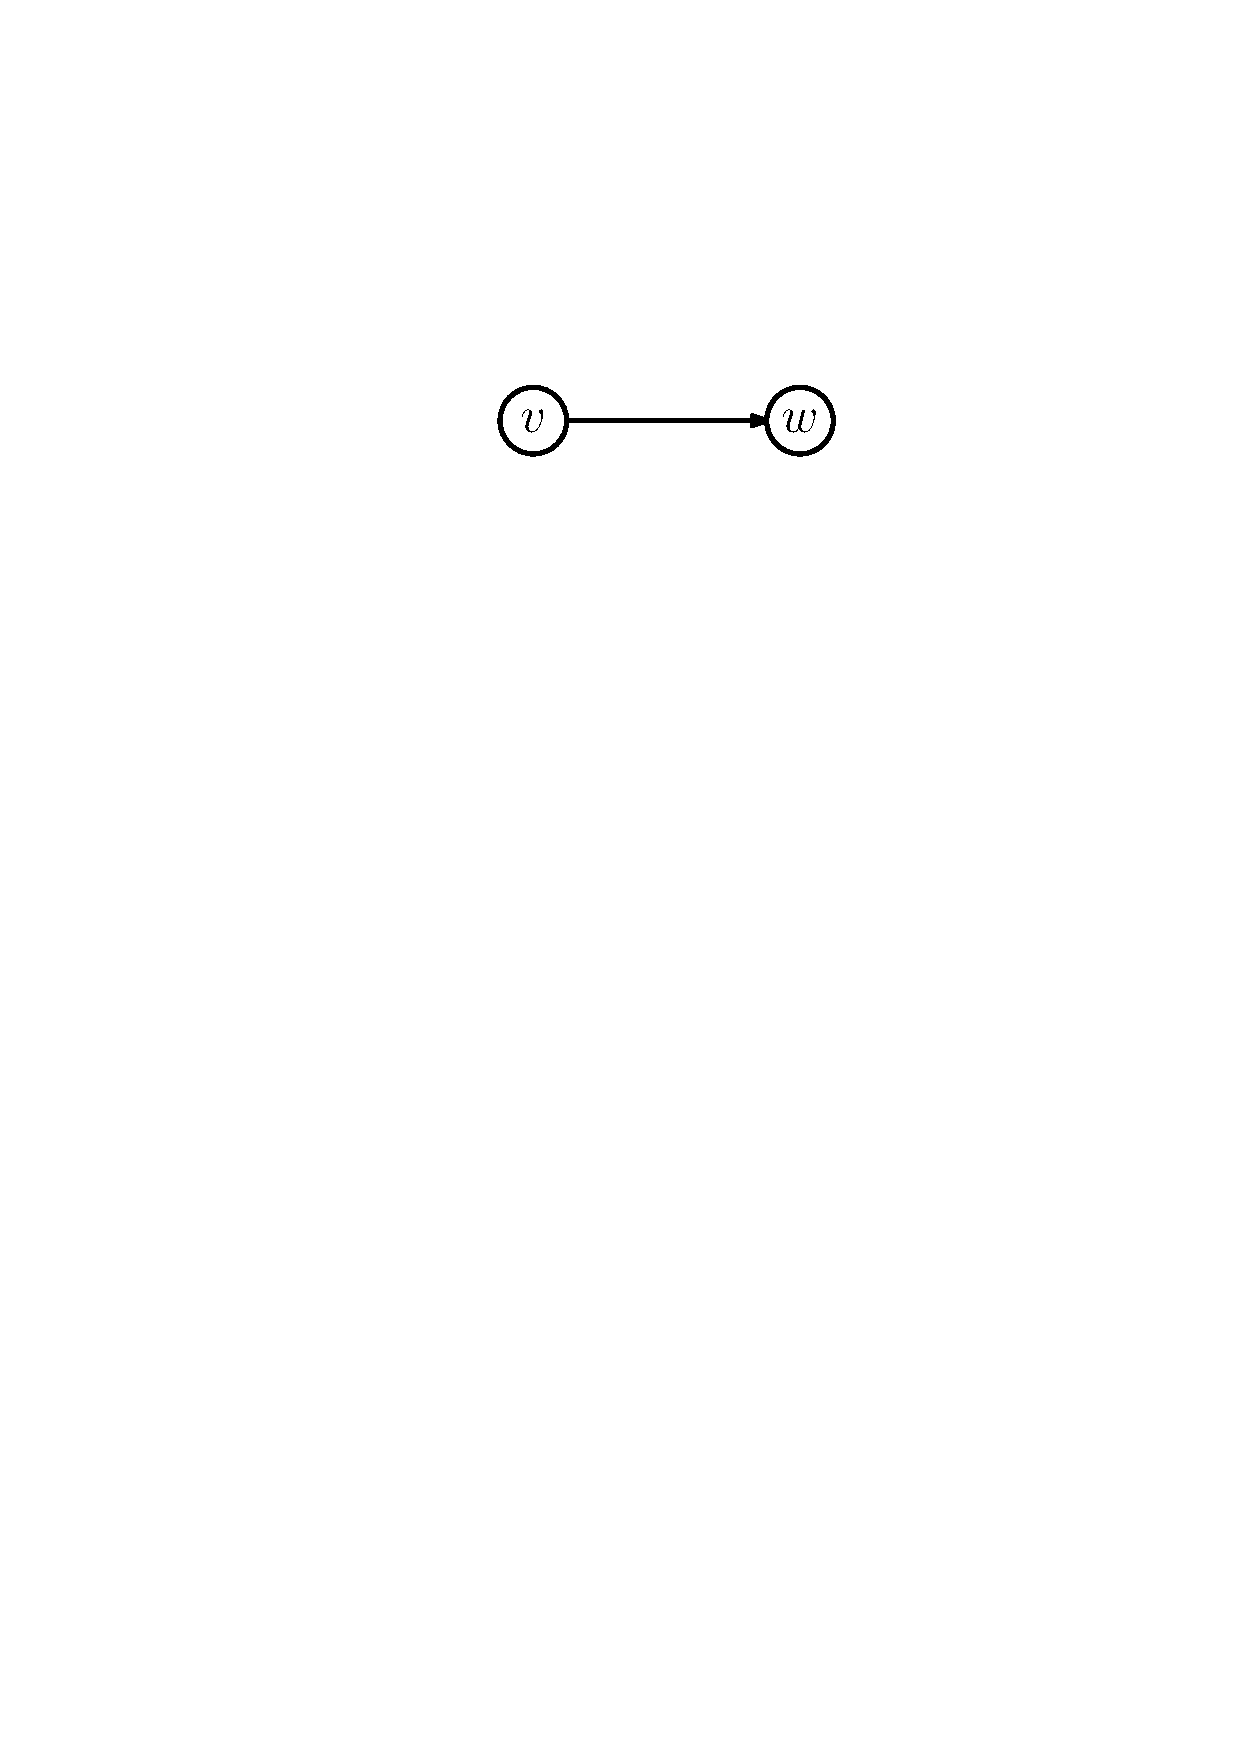
\includegraphics[scale=.5]{01_graph_theory/pics/directed-graph_edge.pdf}
} &
\subfigure[undirected graph] {
	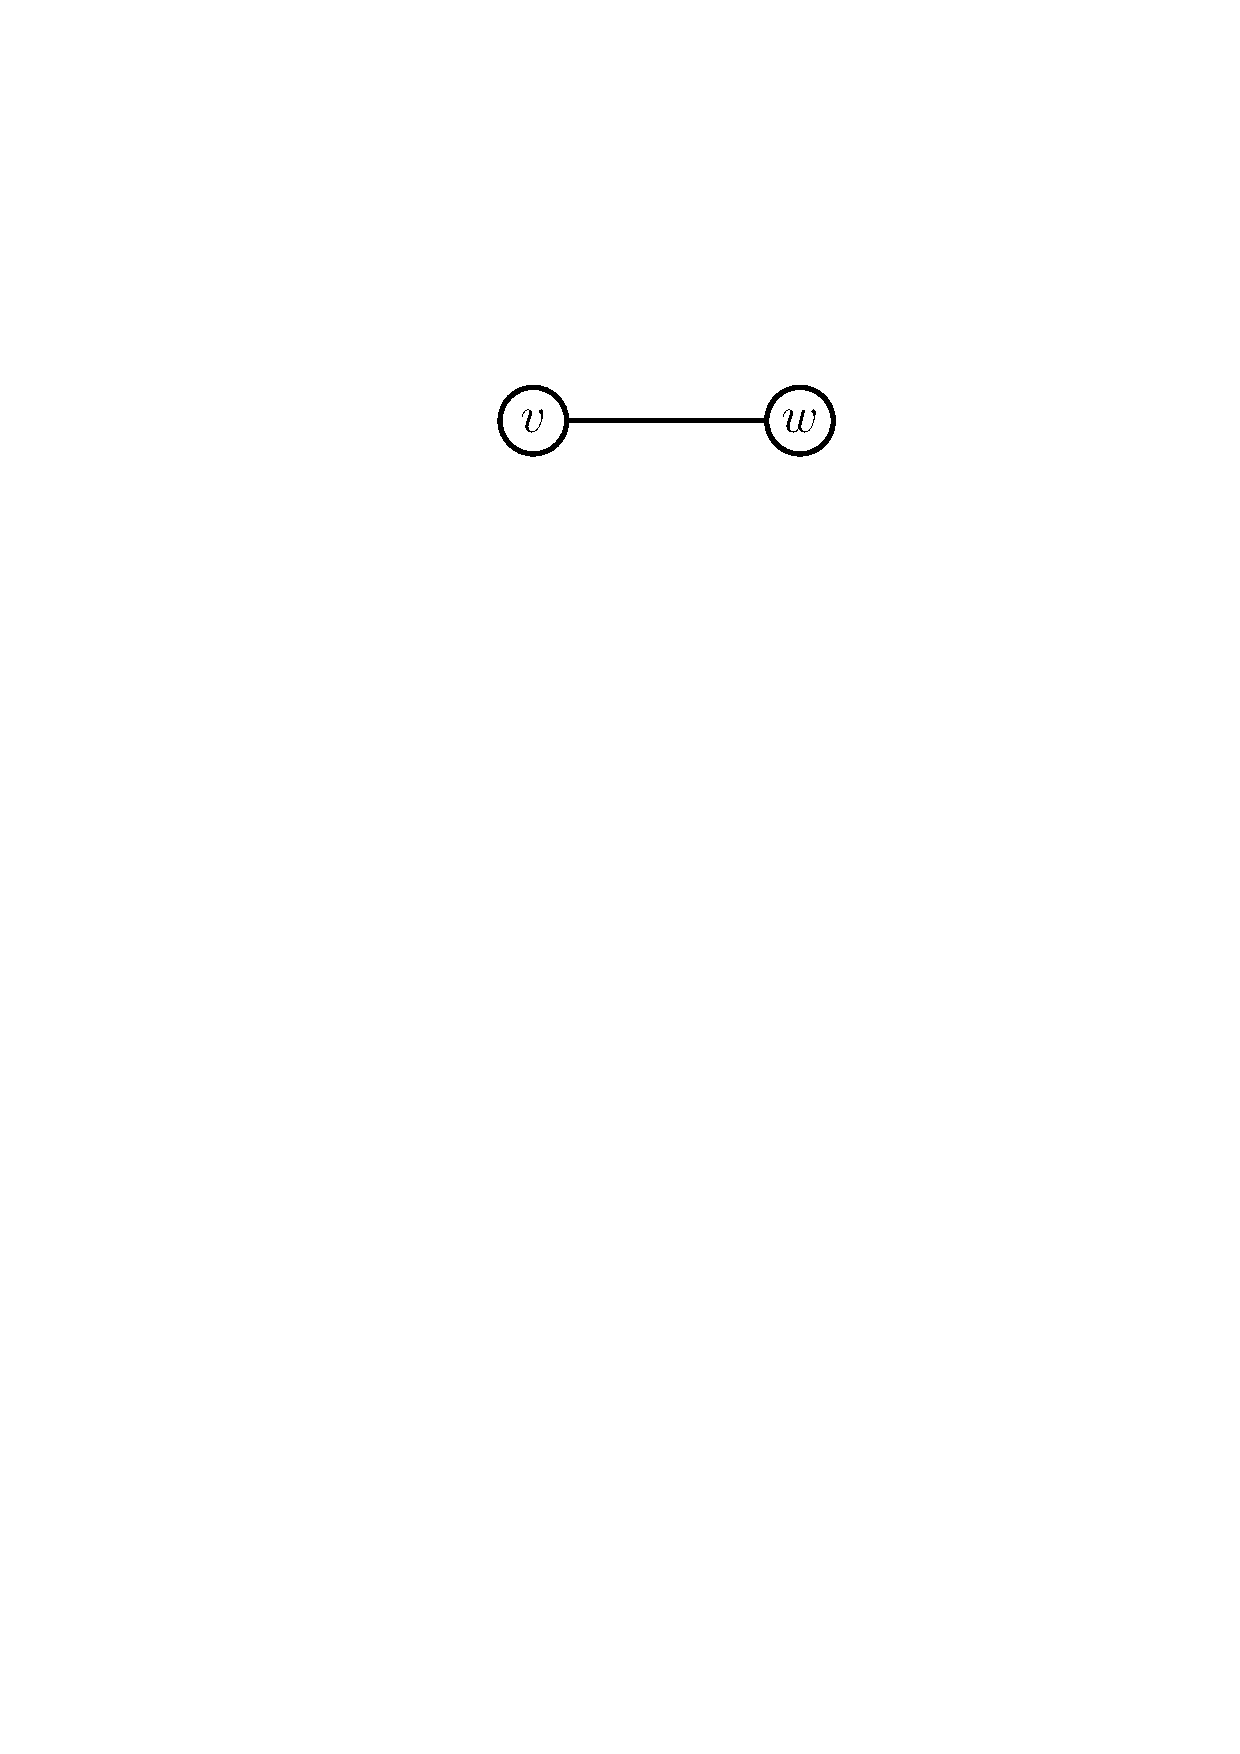
\includegraphics[scale=.5]{01_graph_theory/pics/graph_edge.pdf}
} \\
\subfigure[loop] {
	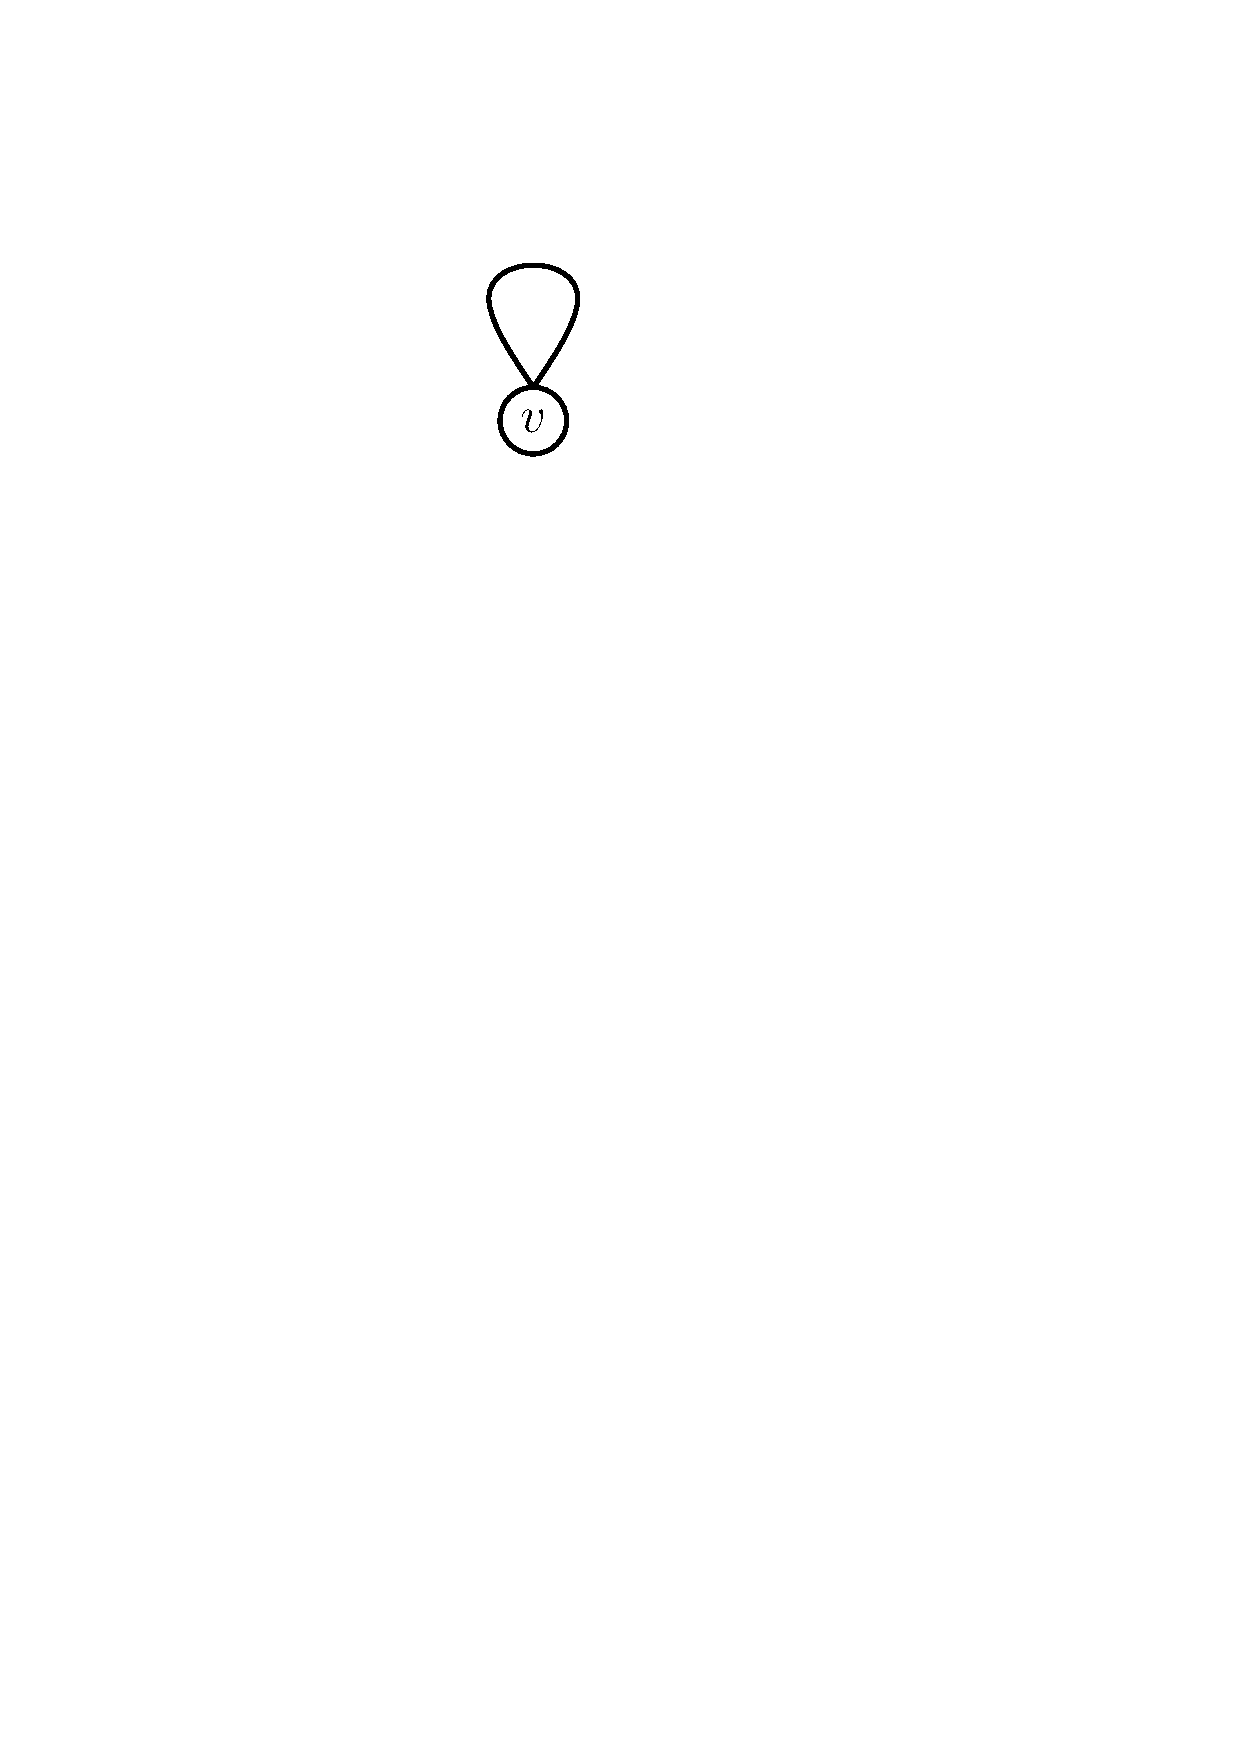
\includegraphics[scale=.5]{01_graph_theory/pics/graph_loop.pdf}
} &
\subfigure[multiple edges] {
	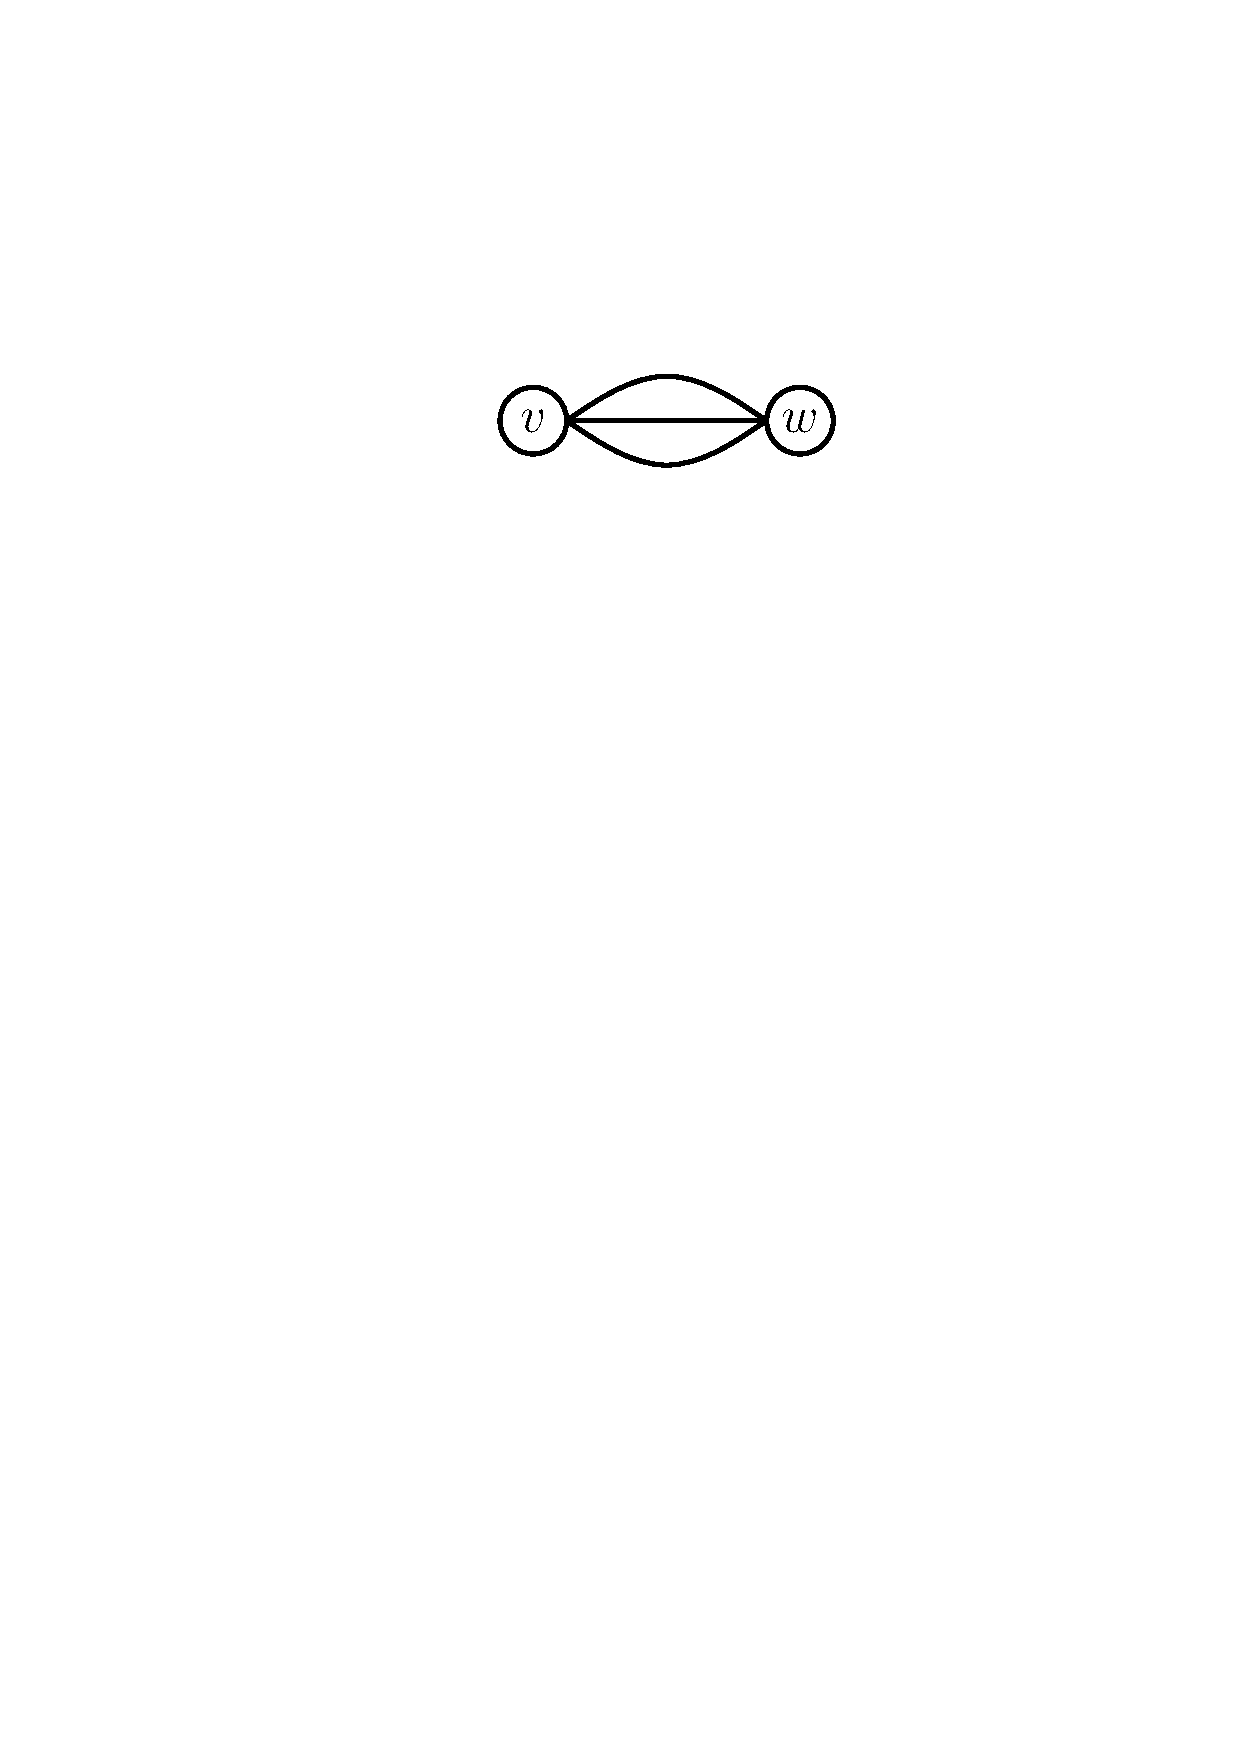
\includegraphics[scale=.5]{01_graph_theory/pics/graph_multiple-edges.pdf}
}
\end{tabular}
\caption{different graphs}
\end{figure}
\FloatBarrier

\begin{definition}
\index{graph!simple}
A graph is \dt{simple} when it has
\begin{compactitem}
\item no loops and
\item no multiple edges.
\end{compactitem}
\end{definition}

Unless otherwise stated, we assume simple, finite graphs throughout this
lecture.

A graph corresponds to a \emph{relation} on $V$. In case of undirected graphs,
this relation is symmetric.


Notation: \\[\medskipamount]
\begin{tabular}{ll}
  $V$, $V(G)$ & vertice set \\
  $E$, $E(G)$ & edge set \\
  $\alpha_0 = |V|$ & number of vertices \\
  $\alpha_1 = |E|$ & number of edges \\
\end{tabular}

\begin{definition}
\index{degree}
Let $v\in V$. For undirected graphs,
\begin{compactitem}
  \item the \dt{degree} $d(v)$ is the number of edges \emph{incident} to $v$.
\end{compactitem}
For directed graphs,
\begin{compactitem}
  \item the \dt{out-degree} $d^{+}(v)$ is the number of outgoing edges, i.e. edges of the form $(v,w)$, and
  \item the \dt{in-degree} $d^{-}(v)$ is the number of incoming edges, i.e. edges of the form $(w,v)$.
\end{compactitem}
\end{definition}

\begin{figure}[htb]
\centering
\subfigure[vertex $v$ with degree $d(v)=6$]{
	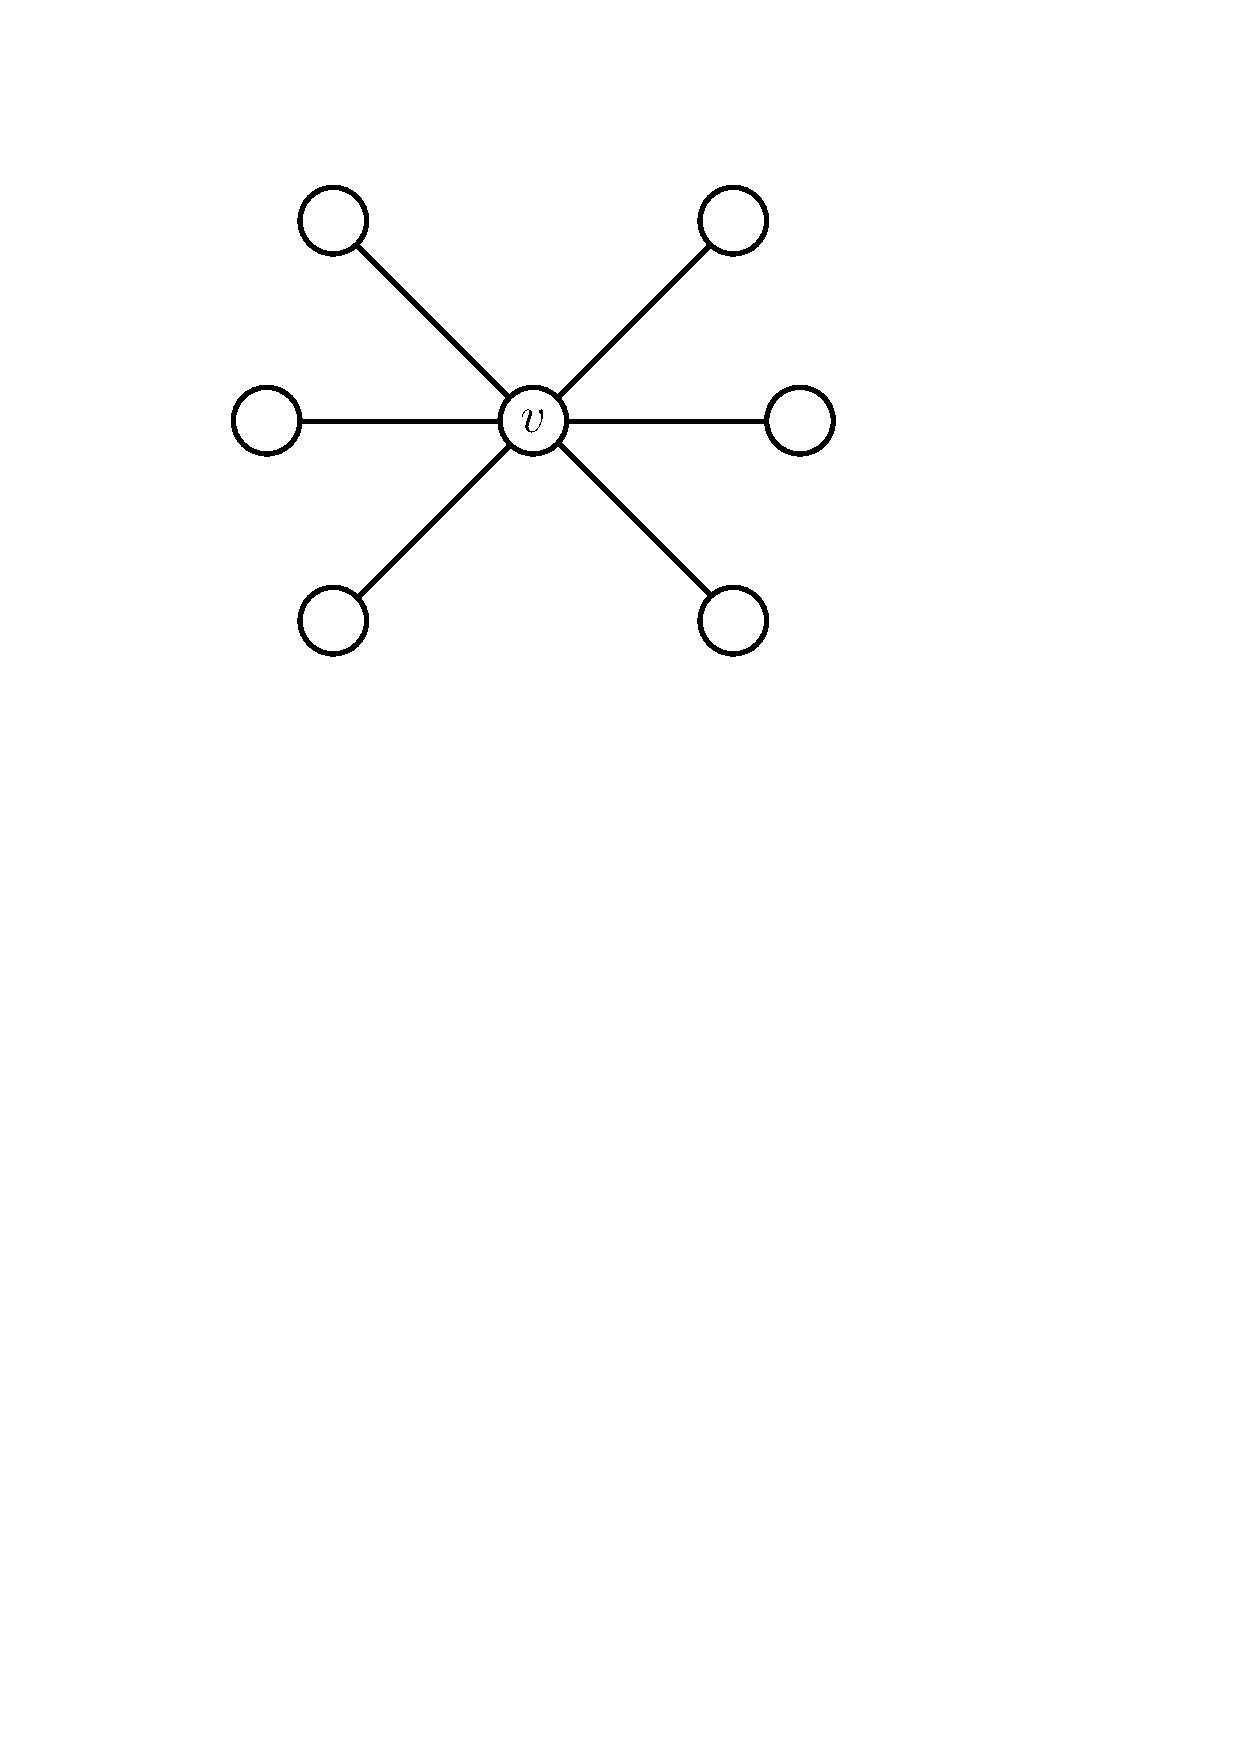
\includegraphics[scale=.5]{01_graph_theory/pics/graph_degree.pdf}
}
\subfigure[vertex $v$ with in-degree $d^{-}(v)=3$ and out-degree $d^{+}(v)=3$]{
	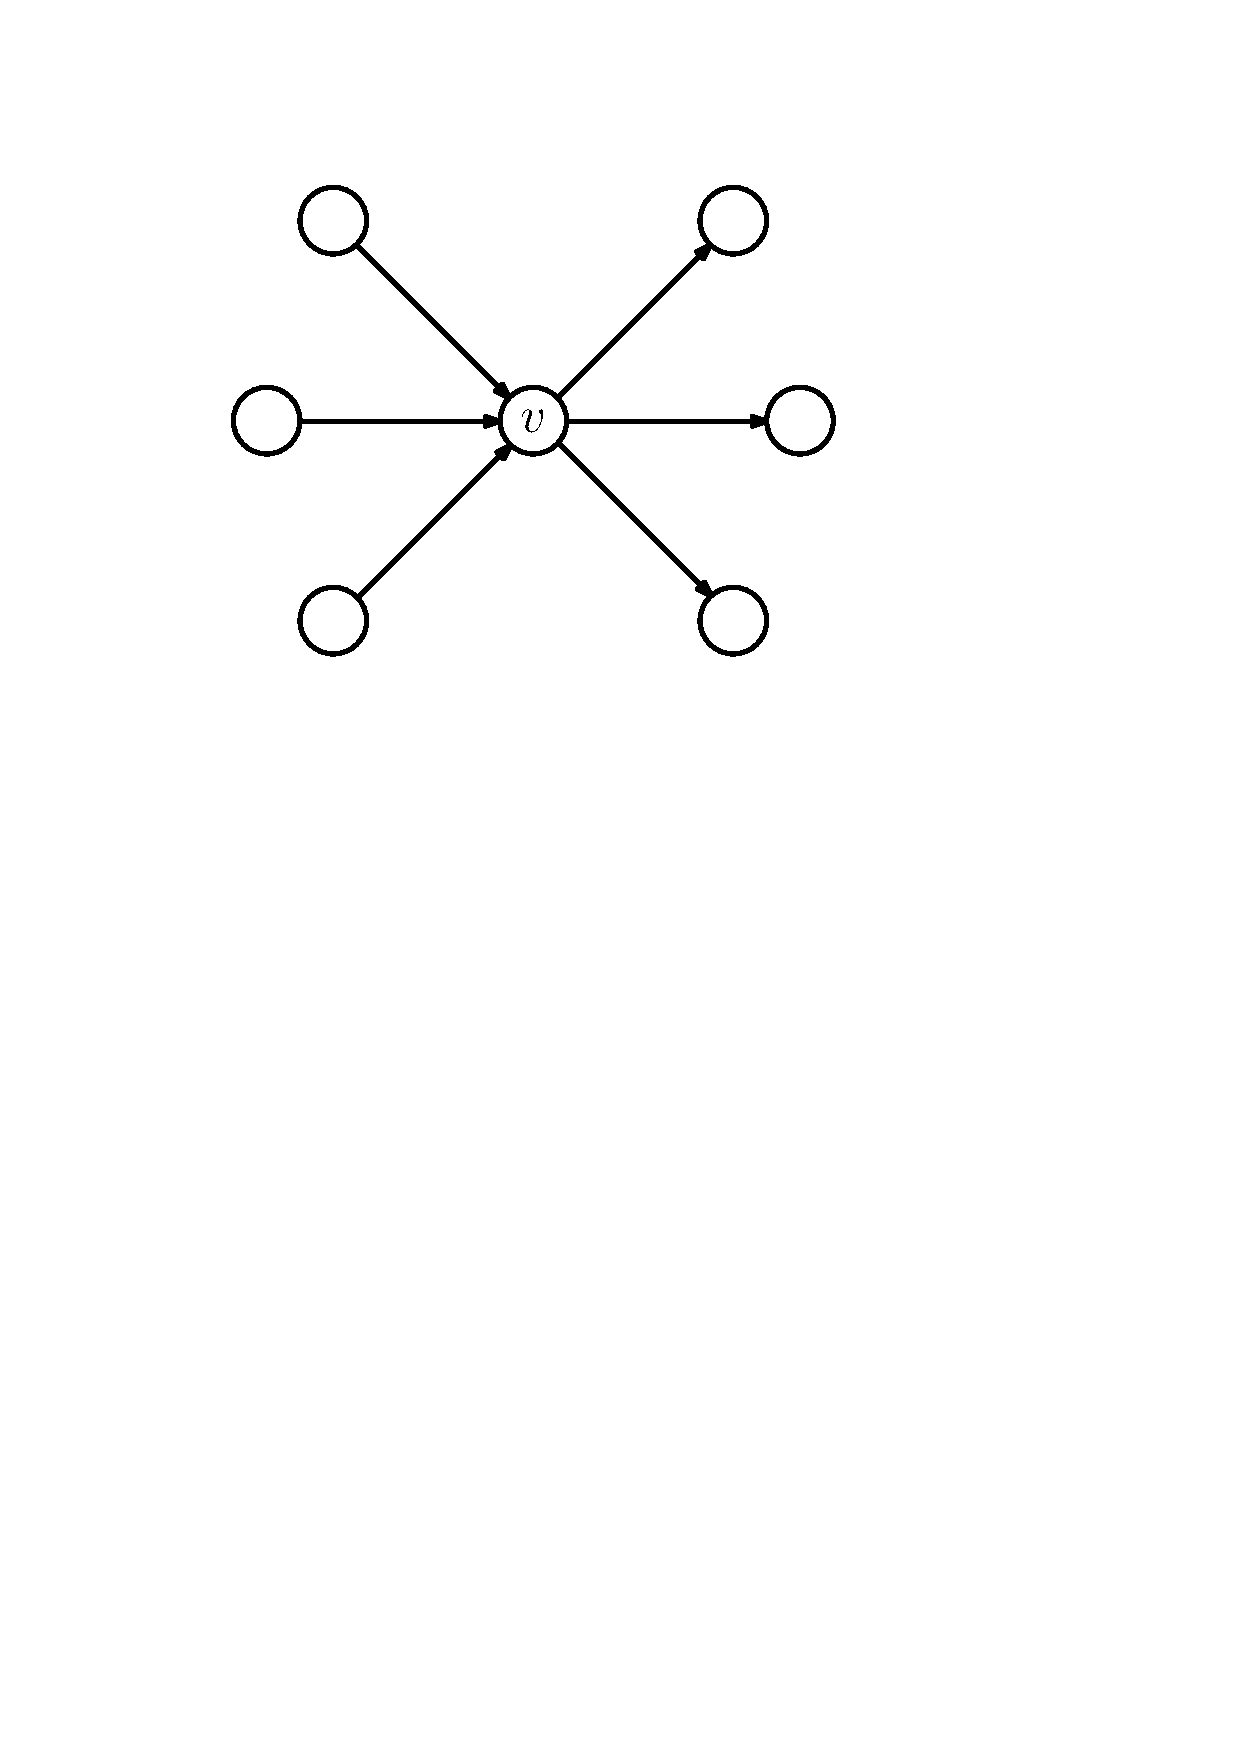
\includegraphics[scale=.5]{01_graph_theory/pics/directed-graph_indegree-outdegree.pdf}
}
\caption{vertex-degrees}
\end{figure}
\FloatBarrier

\begin{definition}
\index{neighbour}
\index{successor}
\index{predecessor}
For undirected graphs,
\begin{compactitem}
\item $\Gamma(v)$ is the \dt{set of neighbours} of $v$.
\end{compactitem}
For directed graphs,
\begin{compactitem}
\item $\Gamma^{+}(v)$ is the \dt{set of successors} of $v$.
\item $\Gamma^{-}(v)$ is the \dt{set of predecessors} of $v$.
\end{compactitem}
\end{definition}

\index{handshaking lemma}
\textbf{Lemma (Handshaking Lemma).} Let $G=(V,E)$ be a simple graph. Then
\begin{align*}
&\sum_{v\in V} d(v) = 2 |E| &&\text{($G$ undirected)} \\
&\sum_{v\in V} d^{+}(v) = \sum_{v\in V} d^{-}(v) = |E| &&\text{($G$ directed).} \\
\end{align*}

\textbf{Proof.} see Figure~\ref{fig:hand_shaking_lemma}

\begin{figure}[htb]
\centering
\subfigure[undirected graph, each edge is counted twice]{
	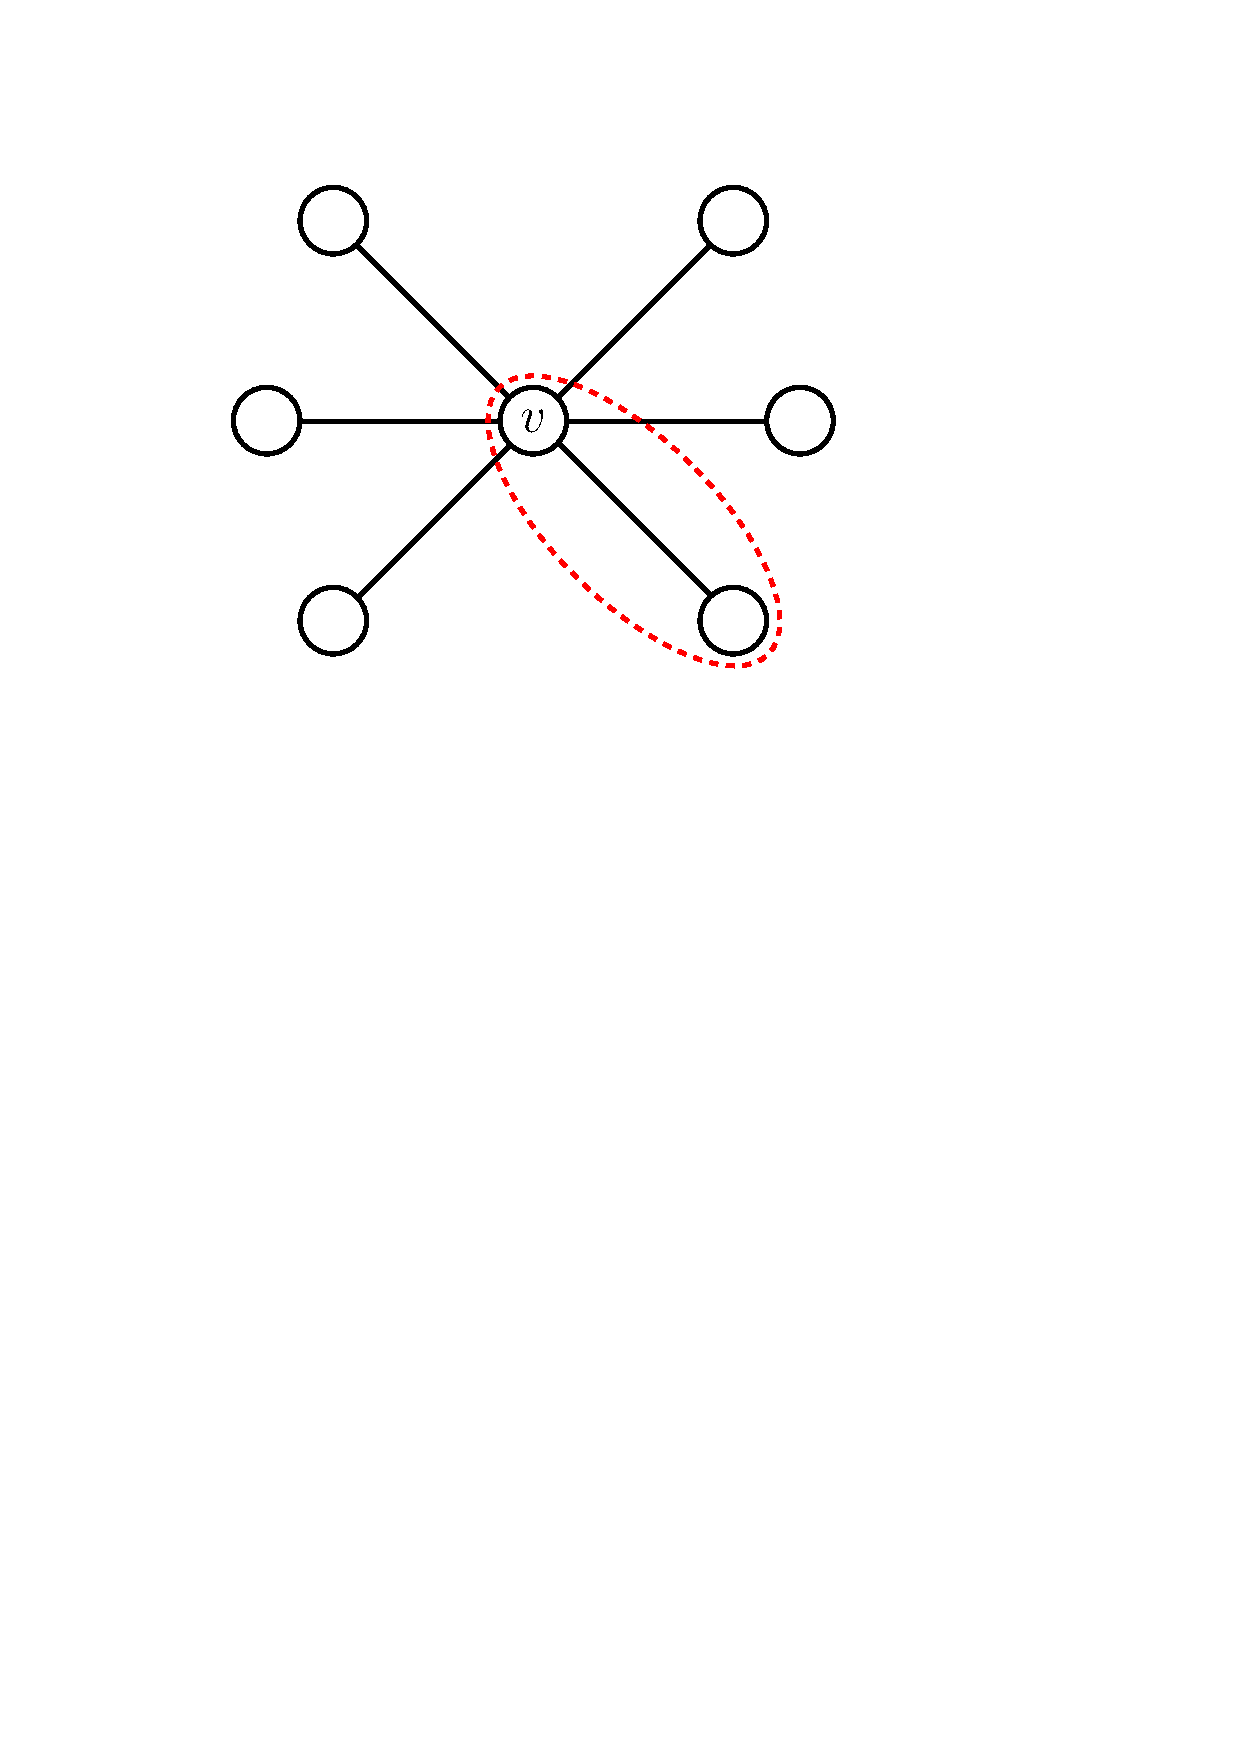
\includegraphics[scale=.5]{01_graph_theory/pics/graph_degree_handshaking-lemma.pdf}
}
\subfigure[directed graph, each edge is counted only once]{
	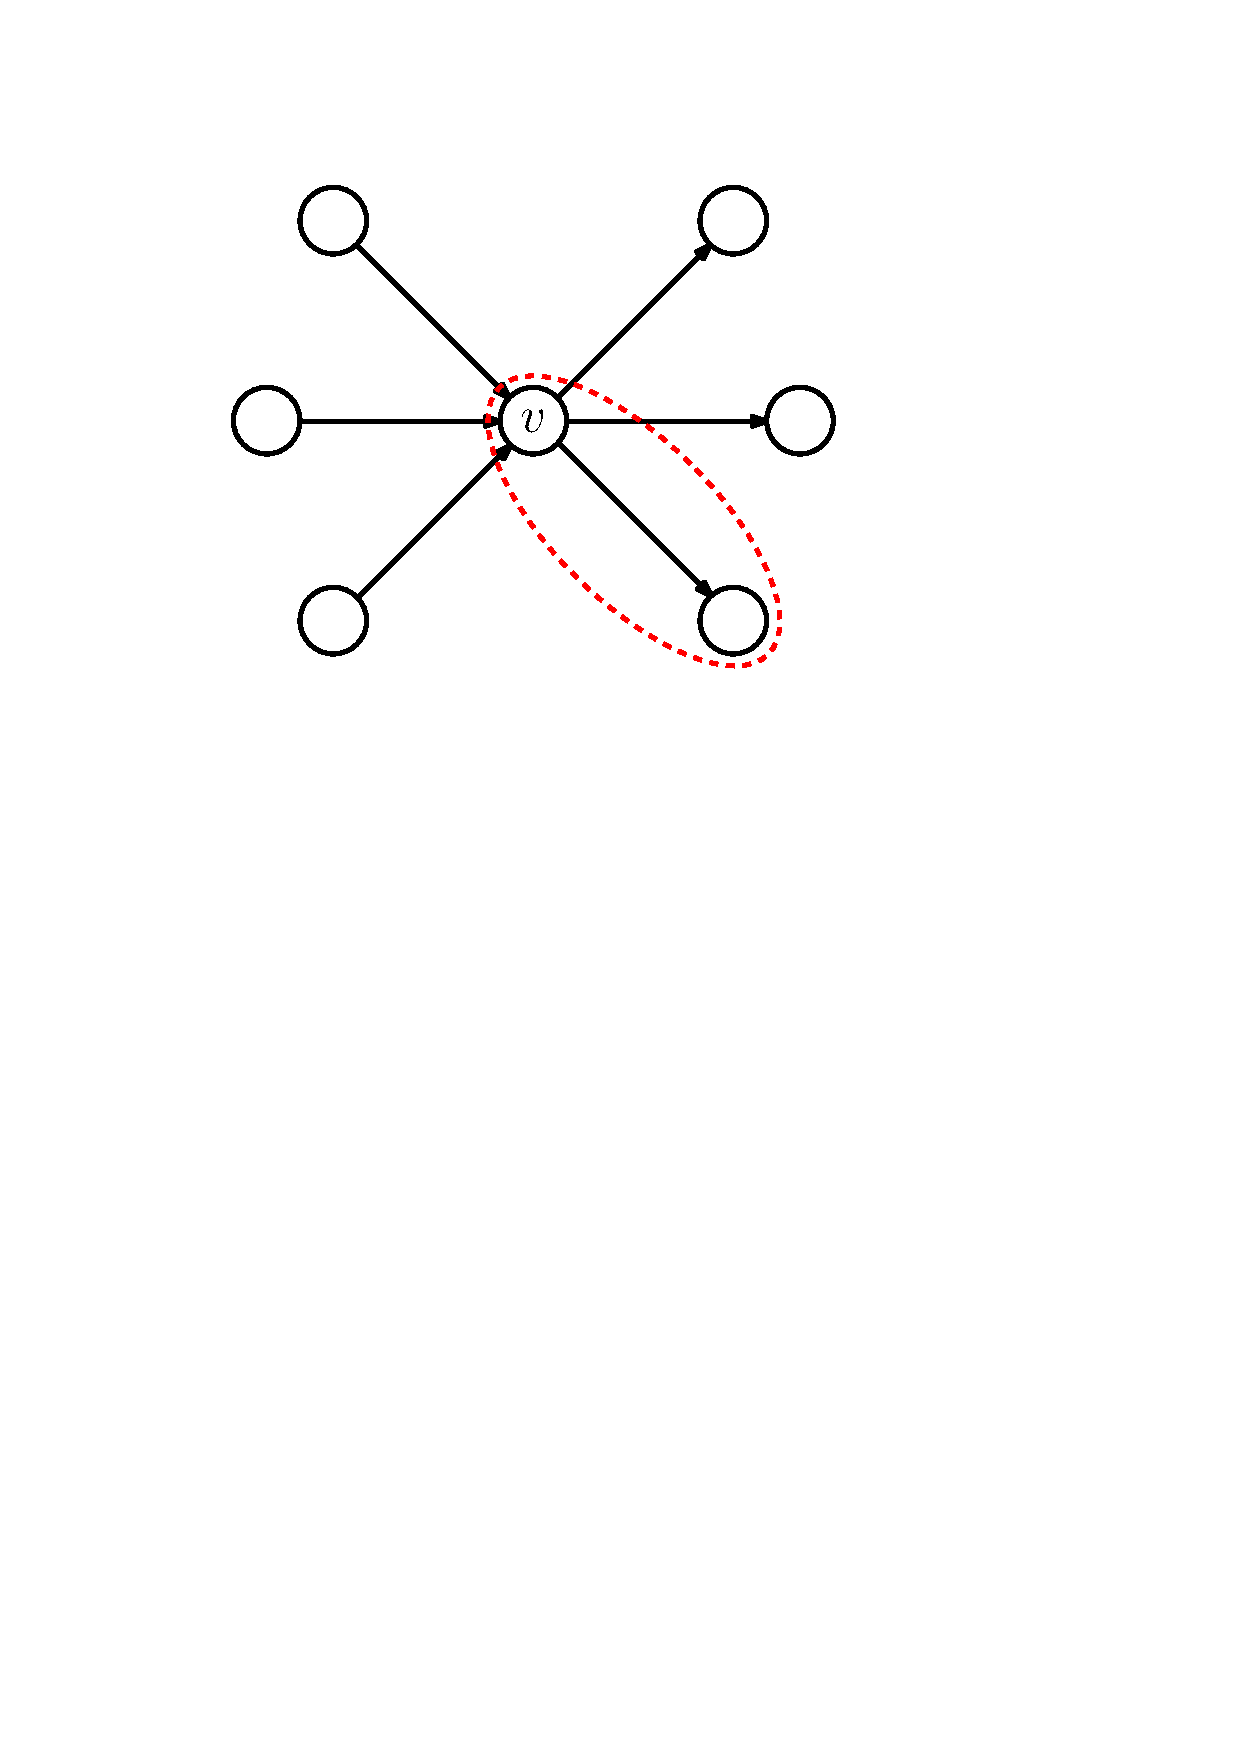
\includegraphics[scale=.5]{01_graph_theory/pics/directed-graph_degree_handshaking-lemma.pdf}
}
\caption{Hand Shaking Lemma in undirected and directed graphs}
\label{fig:hand_shaking_lemma}
\end{figure}
\FloatBarrier

\textbf{Example (Hypercube).}
$G = (\{0,1\}^n, E)$

$vw \in E \Leftrightarrow \sum_{i=1}^{n} |v_i - w_i | = 1$ (only one switch in coordinates)

$v = v_1, v_2, \ldots , v_n$\\
$w = w_1, w_2, \ldots , w_n$

compute $\alpha_0$ and $\alpha_1$

$\alpha_0 = 2^n$ \\
$\alpha_1 = \frac{1}{2} \sum_{v \in V} d(v) = 2^{n-1} * n$

$d(v) = n \Rightarrow $ regular Graph
\begin{figure}[htb]
\centering
\subfigure[1D-hypercube]{
	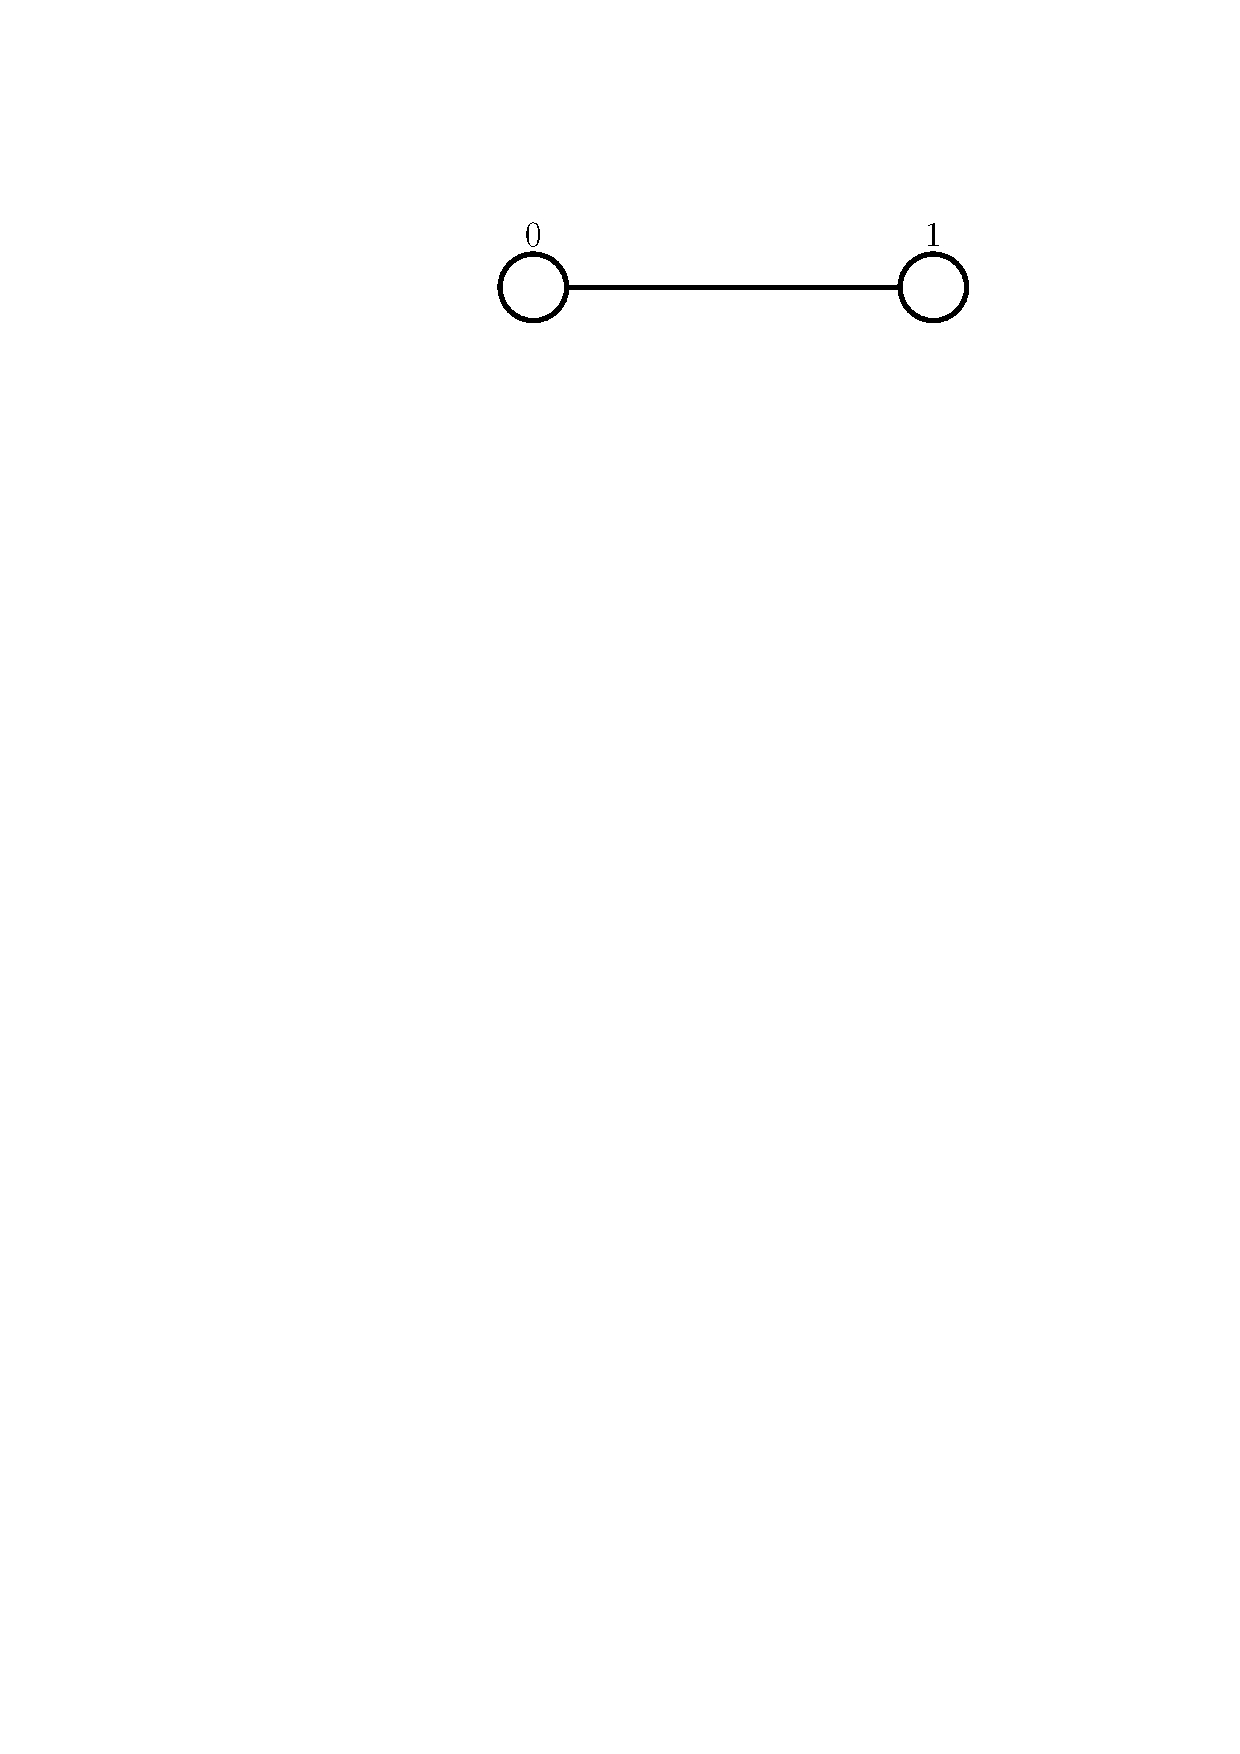
\includegraphics[scale=.4]{01_graph_theory/pics/1D-cube.pdf}
}
\subfigure[2D-hypercube]{
	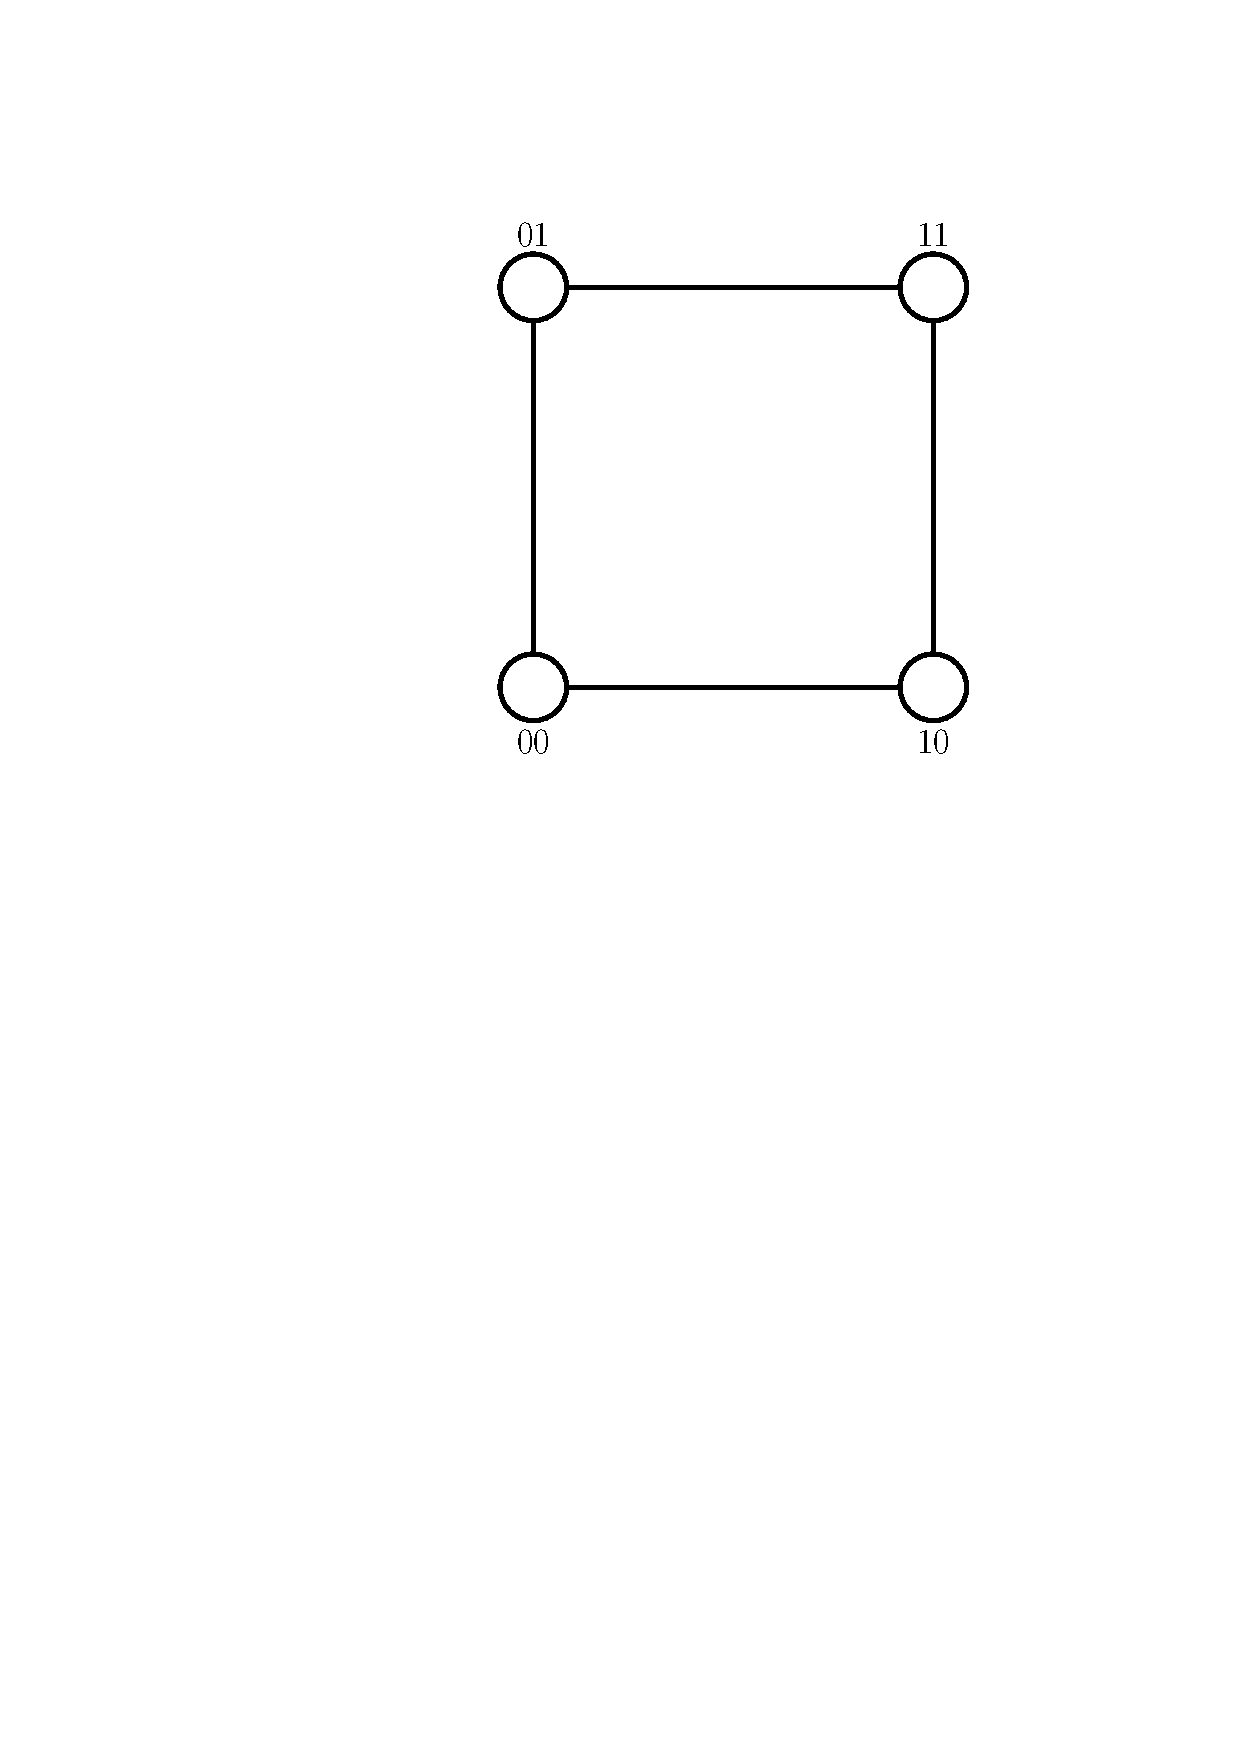
\includegraphics[scale=.4]{01_graph_theory/pics/2D-cube.pdf}
}
\subfigure[3D-hypercube]{
	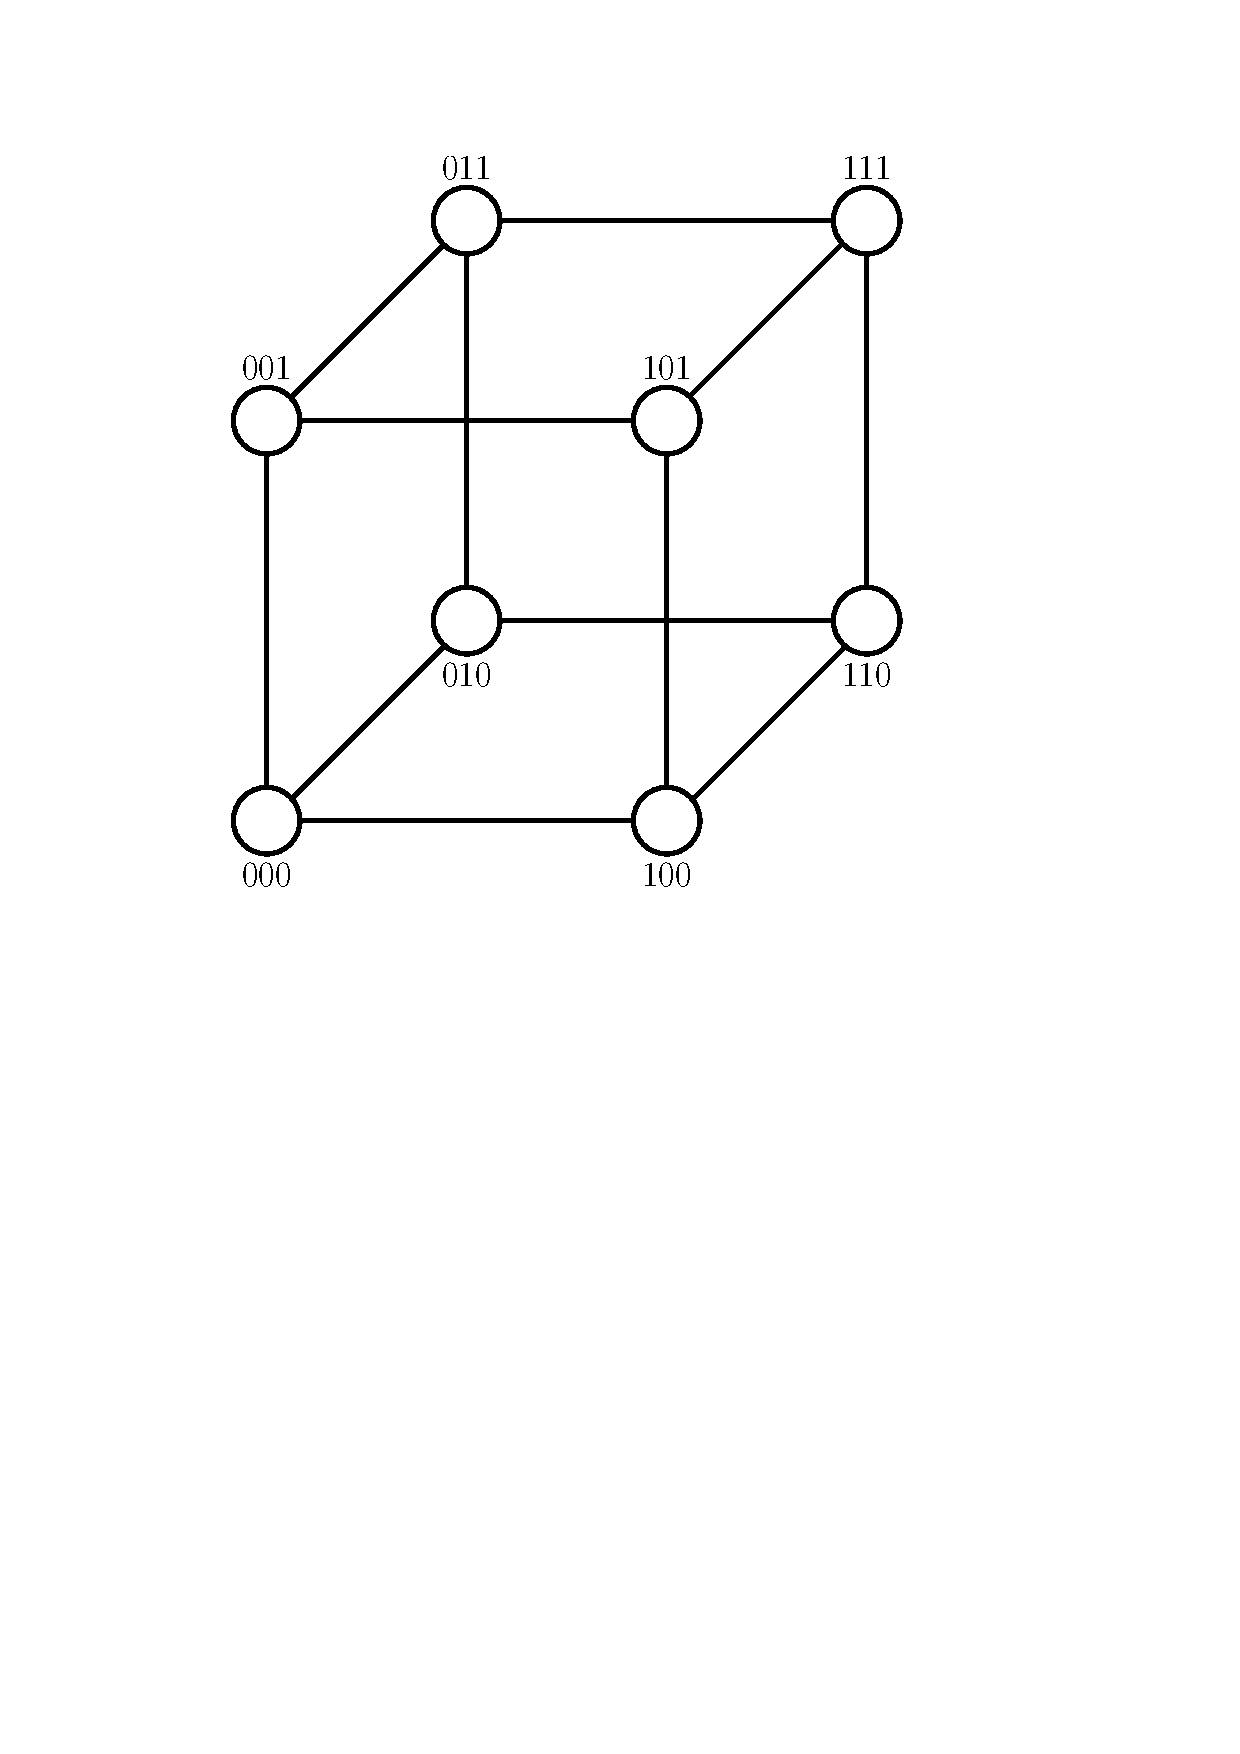
\includegraphics[scale=.4]{01_graph_theory/pics/3D-cube.pdf}
}
\caption{n-Hypercubes}
\end{figure}
\FloatBarrier

\begin{definition}
\index{adjacency}
\index{incidence}
Let $e=vw\in E$. Then we say that
\begin{compactitem}
\item $v$ and $w$ are \dt{adjacent} ($v\sim w$), and
\item $e$ and $v$ are \dt{incident} (as well as $e$ and $w$).
\end{compactitem}
\end{definition}

\begin{definition}
\index{adjacency!matrix}
Let $V=\{v_1,\ldots,v_n\}.$ The \dt{adjacency matrix} $A =
(a_{ij})_{i,j=1,\ldots,n}$ consists of entries
\[
  a_{ij} = \begin{cases}
    1 & v_i\sim v_j\text{ ($v_i$ and $v_j$ adjacent)} \\
    0 & v_i\not\sim v_j
  \end{cases}
\]
\end{definition}

\begin{figure}[htb]
\centering
\subfigure[adjacency $k = 1$]{
	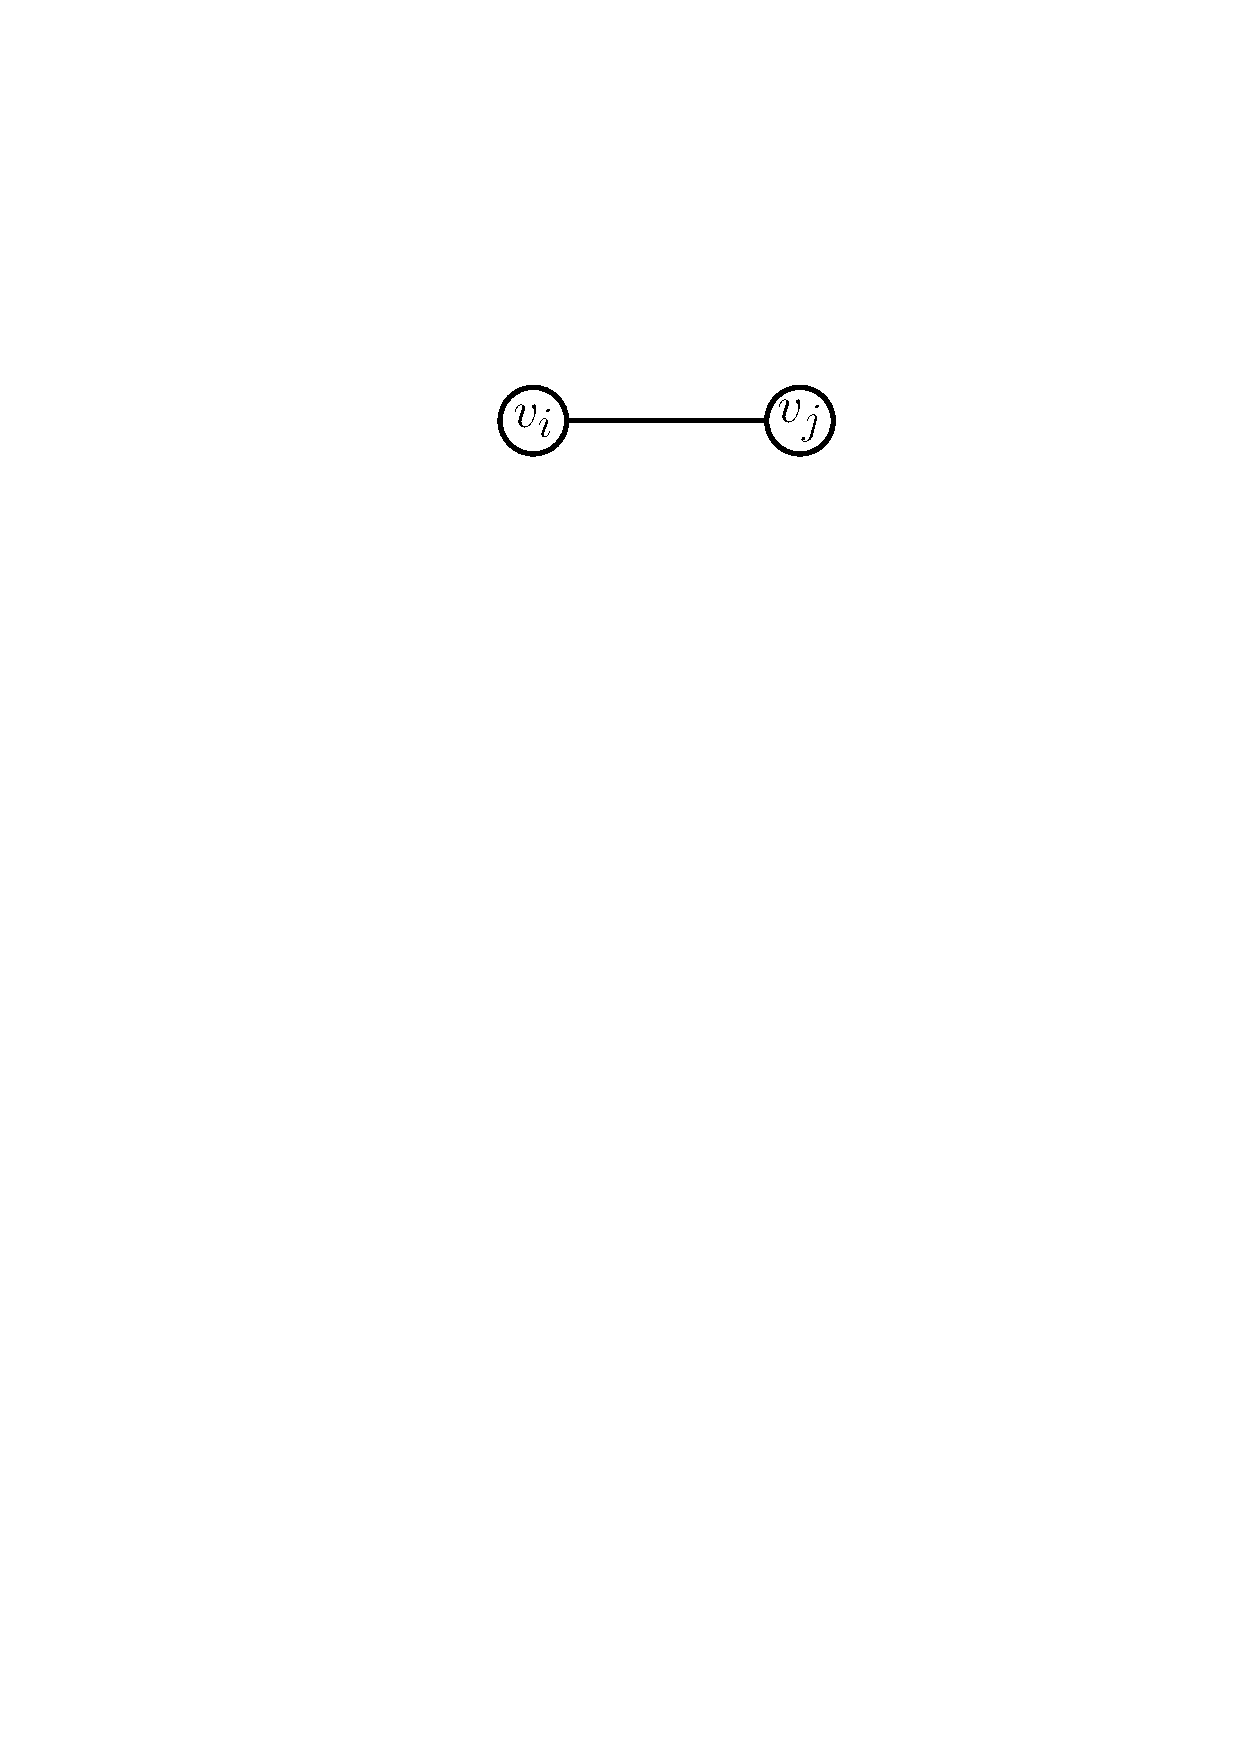
\includegraphics[scale=.5]{01_graph_theory/pics/adjacency_k-1.pdf}
}
\subfigure[adjacency $k = 2$]{
	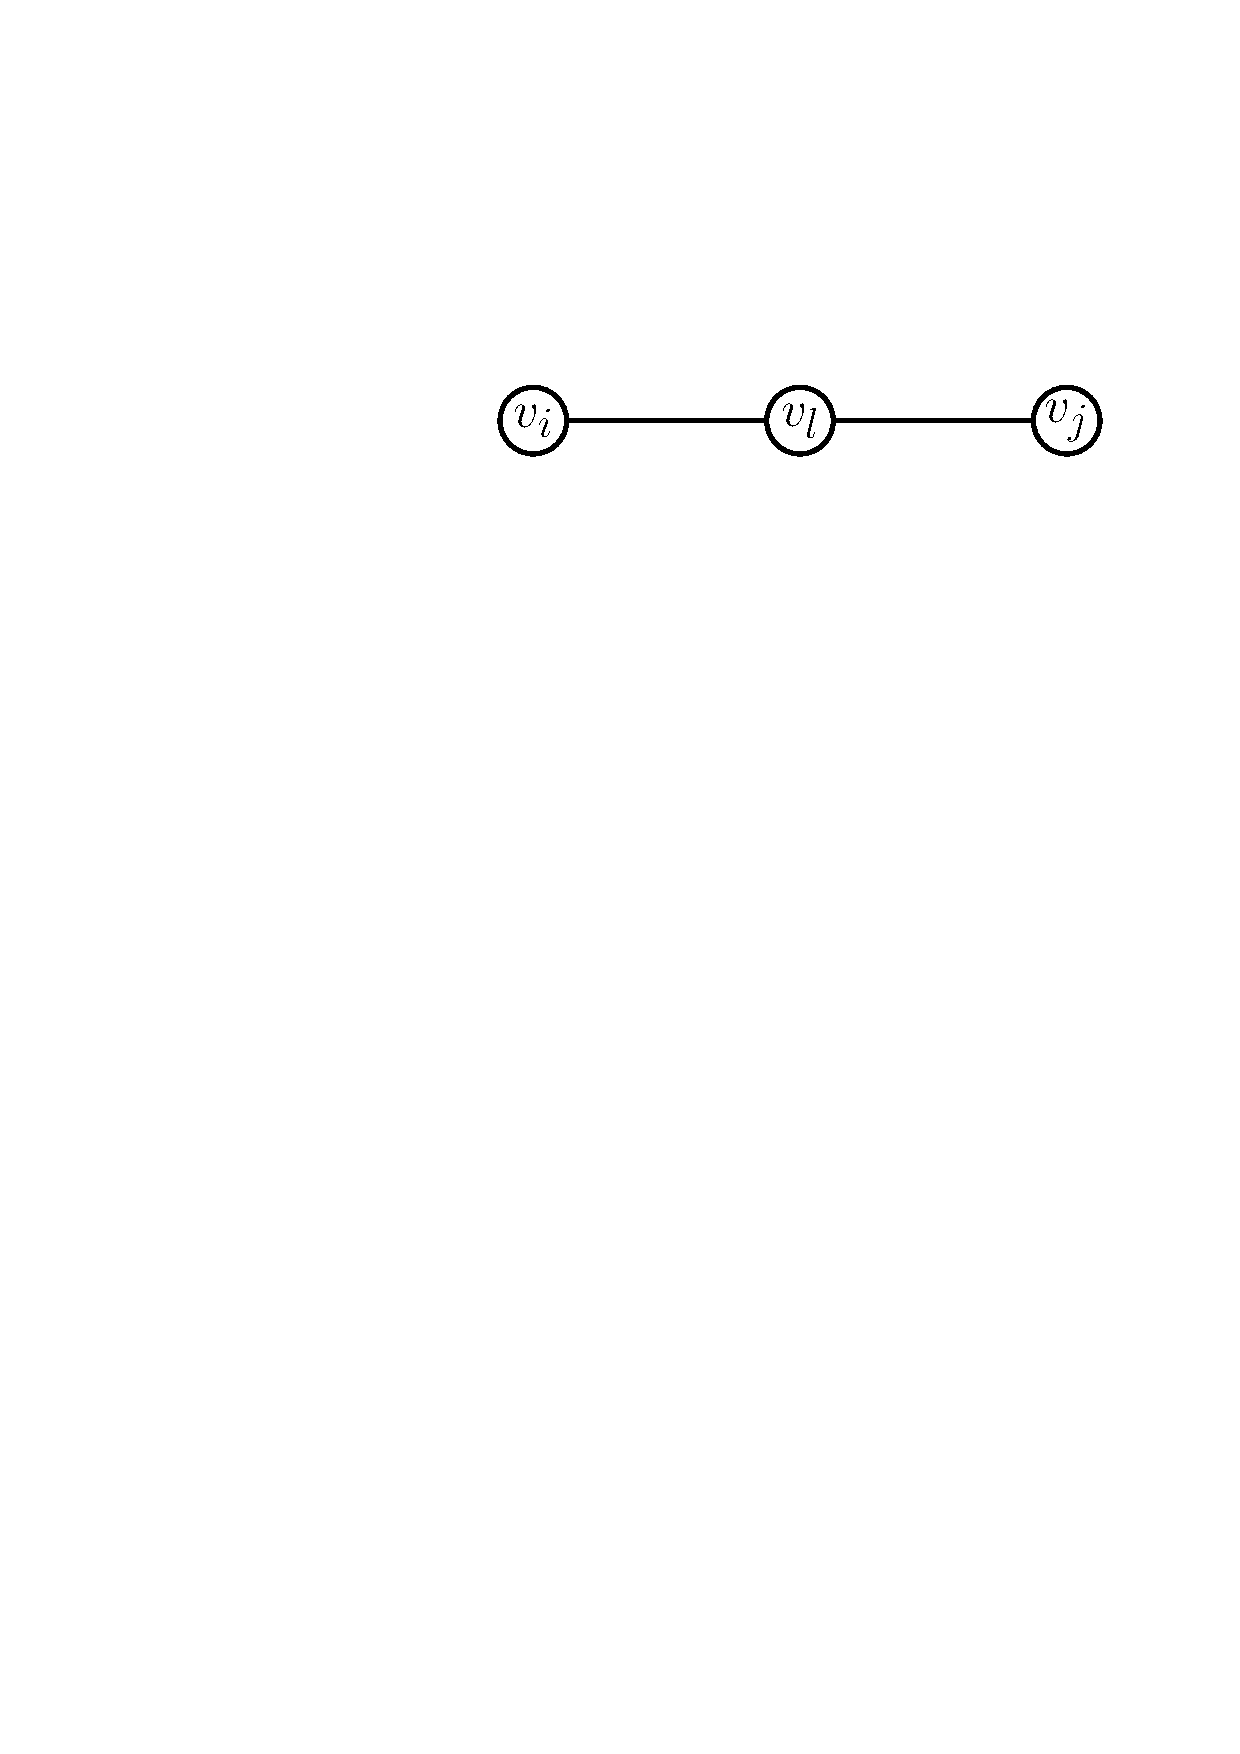
\includegraphics[scale=.5]{01_graph_theory/pics/adjacency_k-2.pdf}
}
\subfigure[adjacency via induction]{
	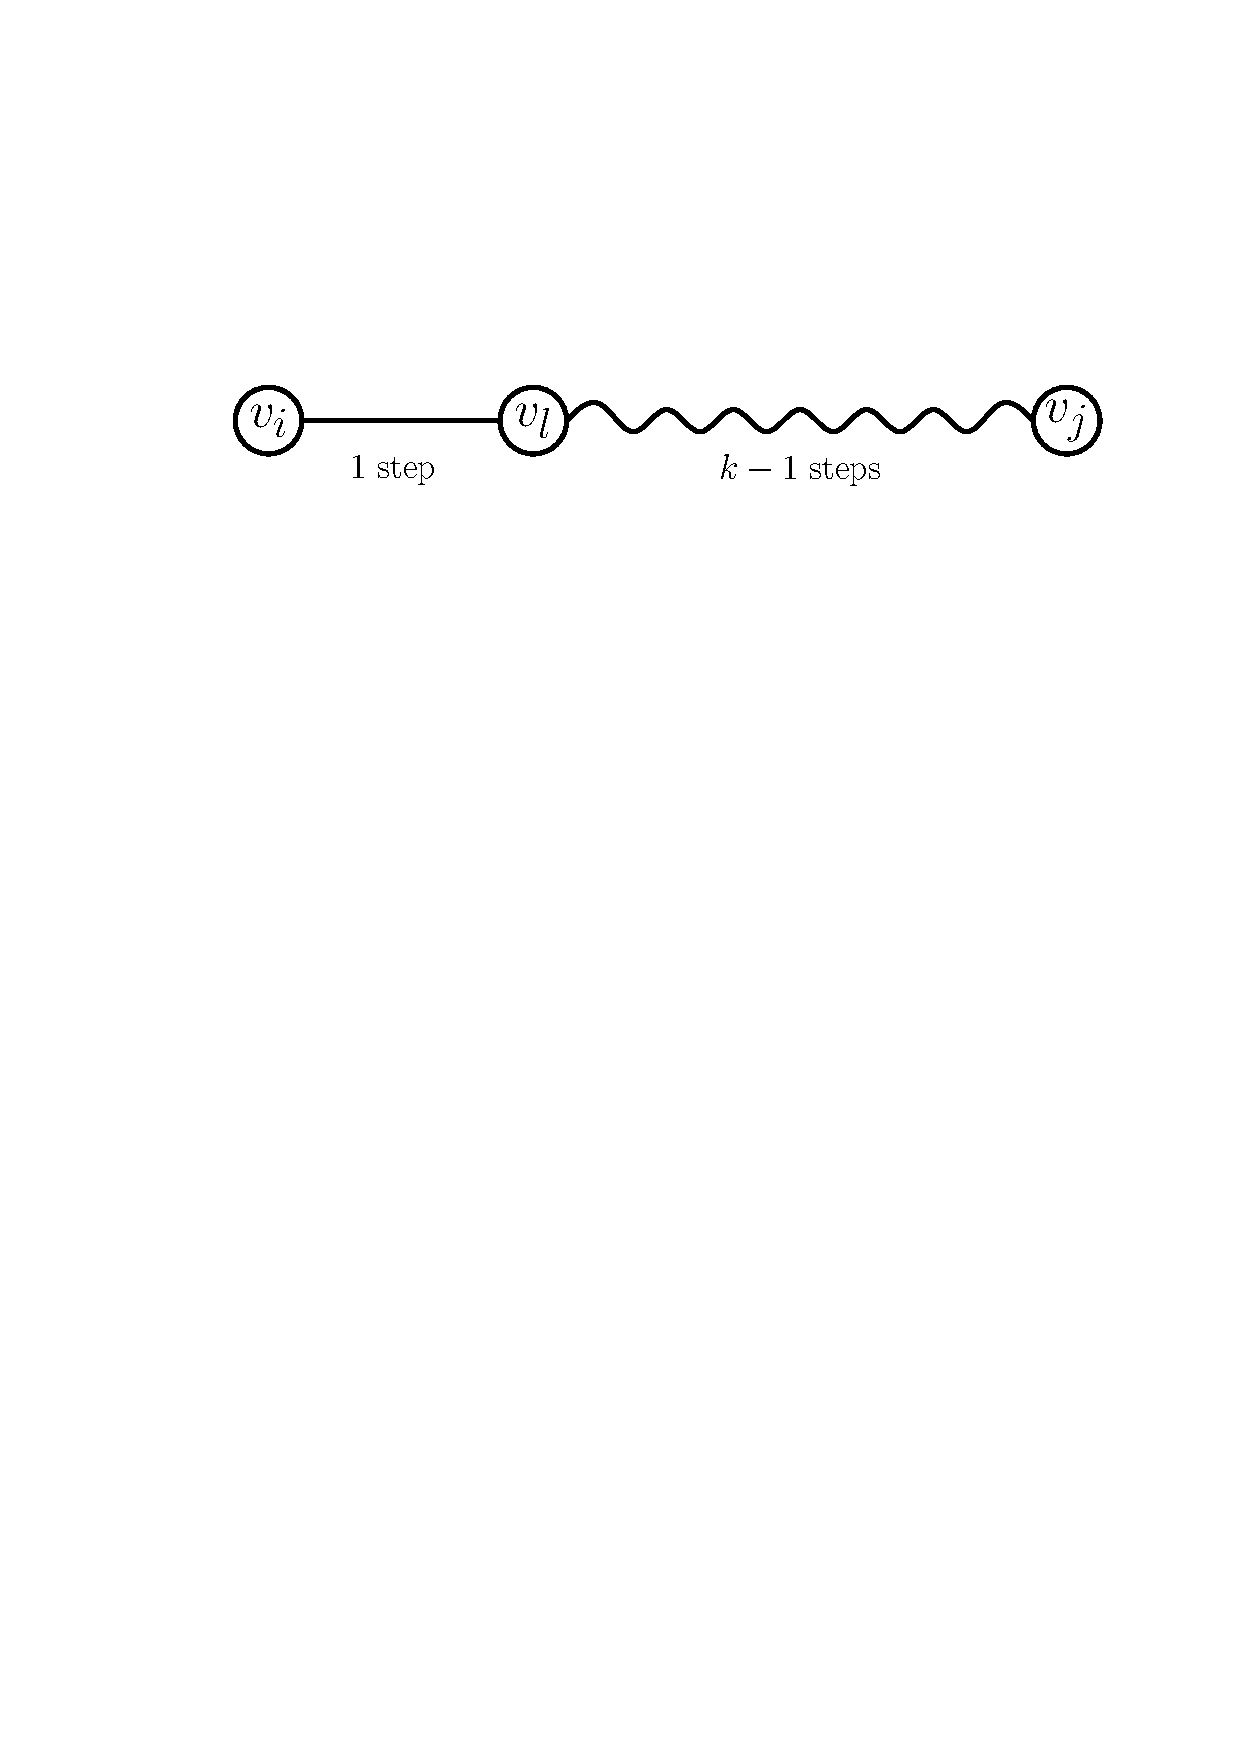
\includegraphics[scale=.5]{01_graph_theory/pics/adjacency_k-induction.pdf}
}
\caption{adjaceny}
\end{figure}
\FloatBarrier

\textbf{Remark.} If $G$ is undirected, $A$ is symmetric.

\textbf{Remark.} Consider
\begin{align*}
A^k &= (a_{ij}^{[k]})_{i,j=1,\ldots,n} = A\cdot A^{k-1} \\
a_{ij}^{[k]} &= \sum_{l=1}^n a_{il}^{\vphantom{[k-1]}}\cdot a_{lj}^{[k-1]}.
\end{align*}
The entries $a_{ij}^{[k]}$ of $A^k$ give the number of ways to get from $v_i$ to $v_j$ in exactly $k$ steps.

\begin{definition}
\index{walk}
A \dt{walk} in a graph $G$ is a sequence of edges, where successive edges have
a vertex in common. Edges can appear multiple times.
\end{definition}

\begin{figure}[htb]
\centering
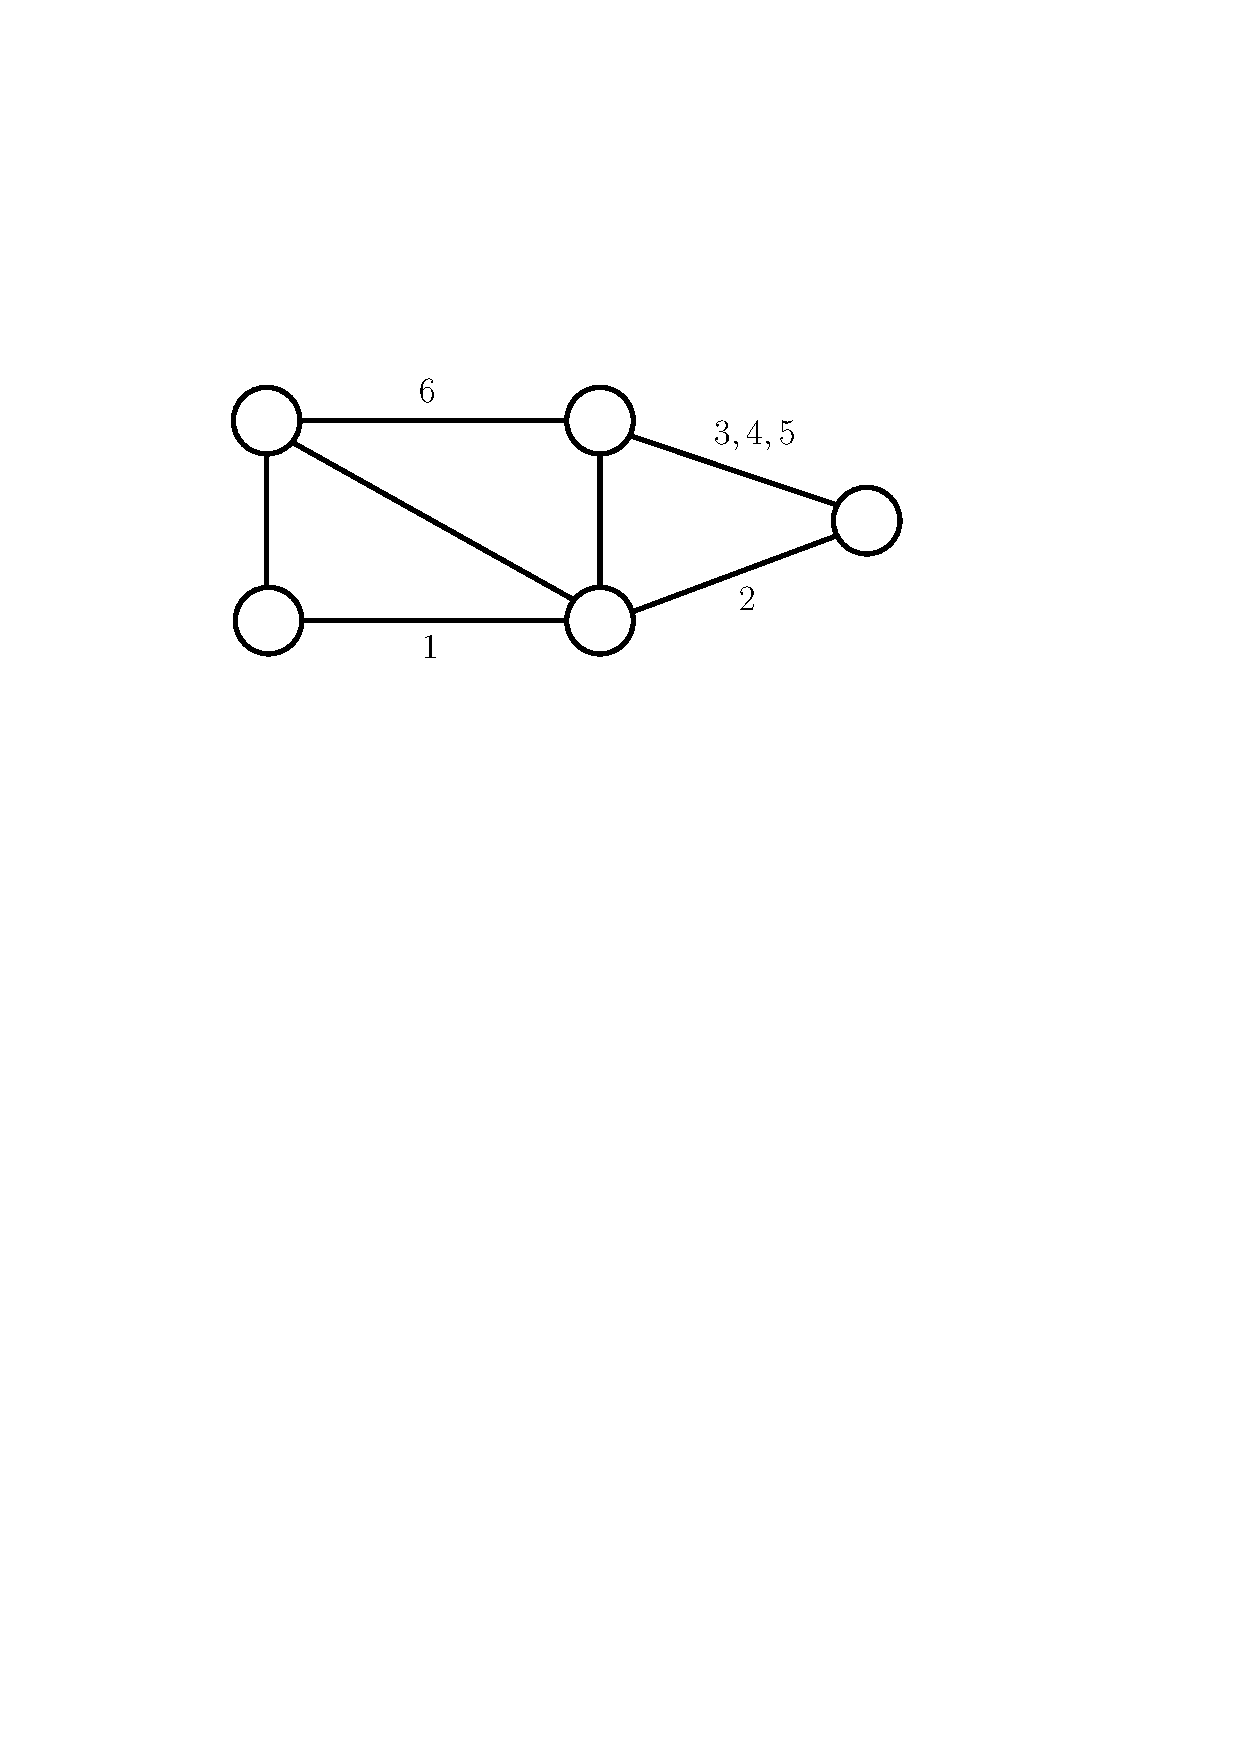
\includegraphics[scale=.5]{01_graph_theory/pics/walk.pdf}
\caption{Example of a walk through a graph}
\end{figure}
\FloatBarrier

\begin{definition}
\index{trail}
\index{circuit}
A \dt{trail} is a walk without repeated edges. A \dt{closed trail} or
\dt{circuit} starts and ends at the same vertex.
\end{definition}

\begin{definition}
\index{subgraph}
Let $G=(V,E)$. $H=(V',E')$ is a \dt{subgraph} of $G$ ($H \leq G$) if
\begin{compactitem}
\item $H$ is a graph,
\item $V' \subseteq V$, and
\item $E' \subseteq E$.
\end{compactitem}
$E'$ only contains edges between vertices in $V'$, this is implied by the requirement that $H$ is a graph.
\end{definition}

\begin{definition}
\index{connectivity}
\index{relation!connectivity relation}
For undirected graphs, we define the \dt{connectivity relation} $\operatorname{R}$ as follows:
\[ v \operatorname{R} w \text{ ($v$ connected to $w$)} \iff \exists\text{ walk from $v$ to $w$}. \]
\end{definition}

Let
\[ C = \sum_{k=0}^L A^k = (c_{ij})\qquad L = \min(|E|, |V|-1) \]
where $c_{ij}$ gives the number of walks from $v_ii$ to $v_j$ of length $\leq
L$. Now $M = \operatorname{sgn} C$ shows us which vertices are connected.

We observe that
\begin{compactitem}
\item $\forall v\in V: v \operatorname{R} v$,
\item $\forall v,w\in V: v \operatorname{R} w \implies w \operatorname{R} v$, and
\item $\forall v,w,u\in V: v \operatorname{R} w \wedge w \operatorname{R} u \implies v \operatorname{R} u$.
\end{compactitem}
\index{relation!equivalence relation}
Thus $\operatorname{R}$ is an \emph{equivalence relation} on $V$.

As an equivalence relation, $\operatorname{R}$ induces a partition of V.
\begin{gather*}
V = V_1 \cup\cdots\cup V_k \\
V_i \cap V_k = \varnothing\quad i\neq j
\end{gather*}
\index{connected component}%
$V_i$ are the \dt{connected components} of $G$.

\begin{figure}[htb]
	\centering
	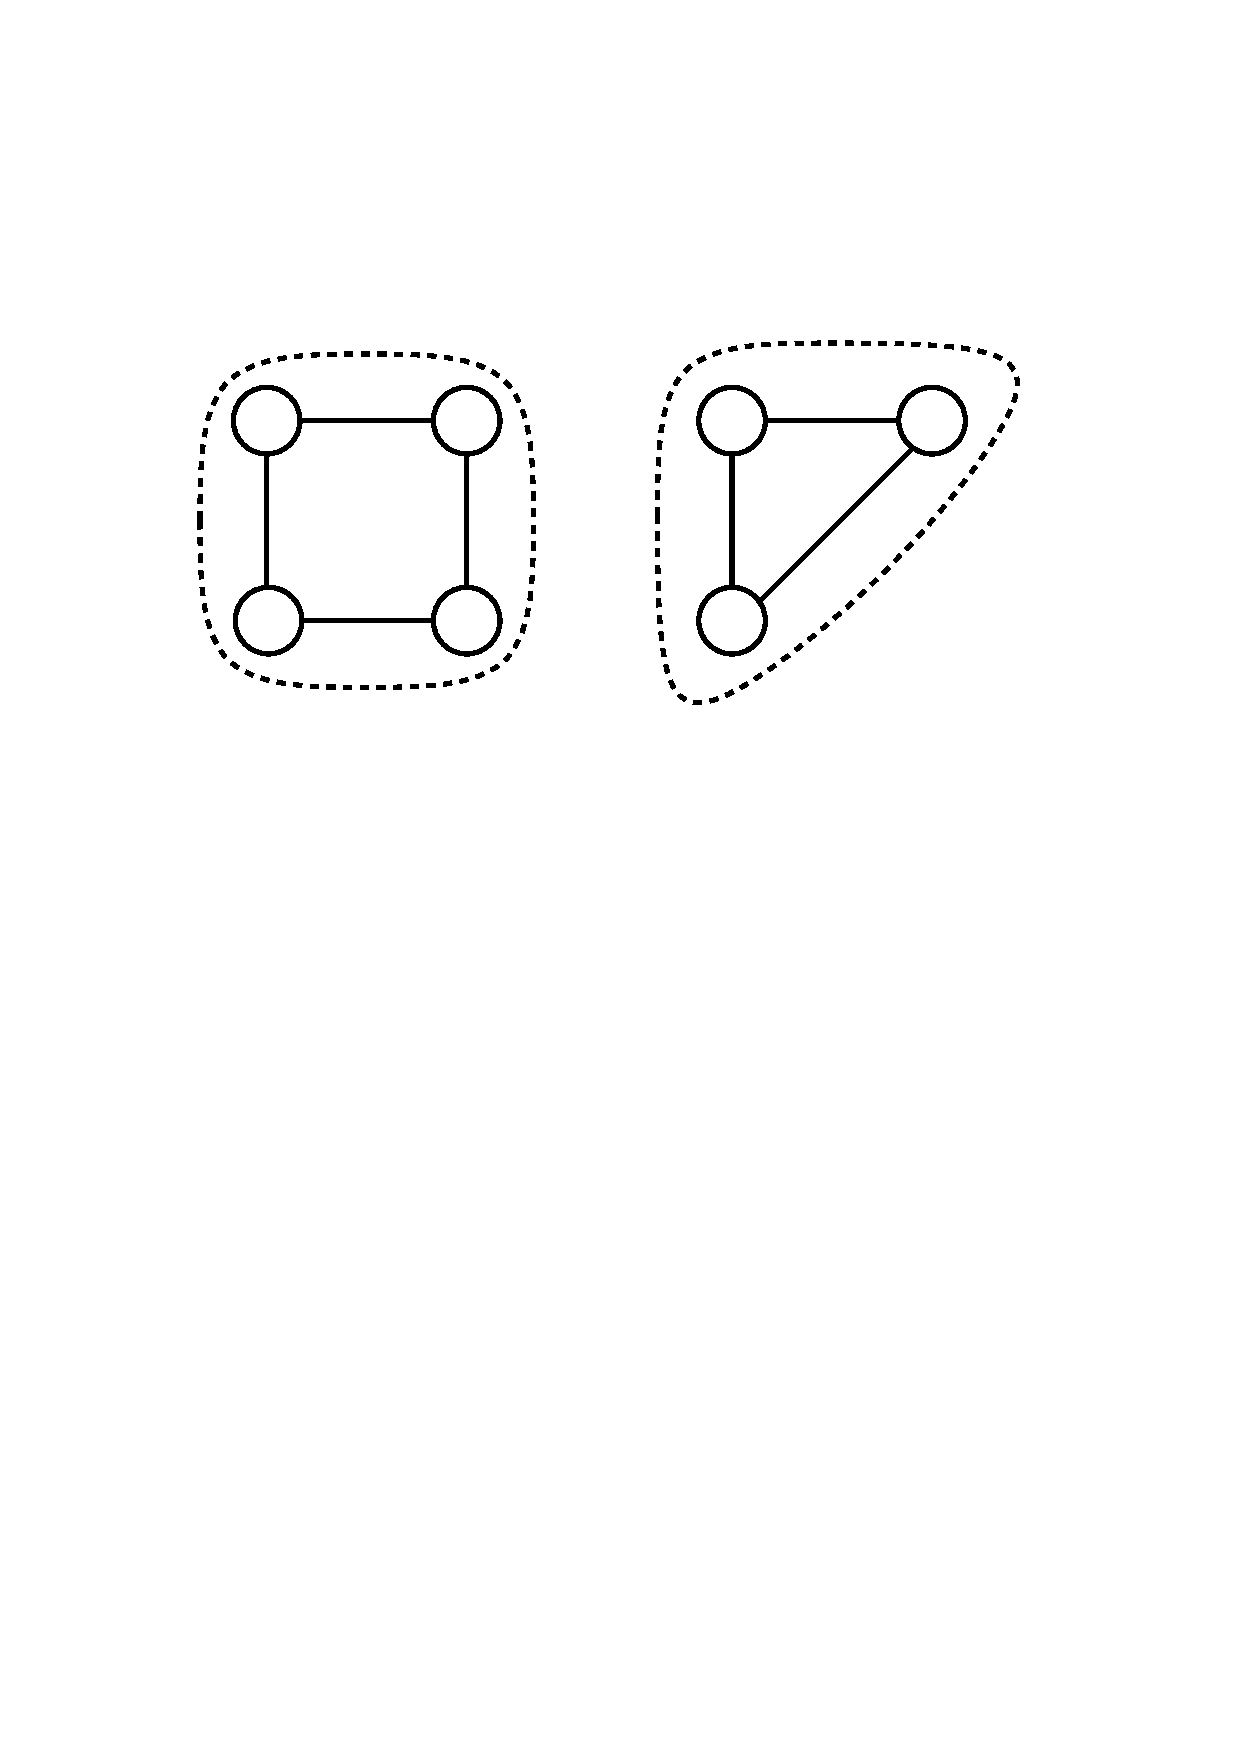
\includegraphics[scale=.5]{01_graph_theory/pics/components.pdf}
	\caption{Graph with 2 components}
\end{figure}
\FloatBarrier

\begin{definition}
\index{graph!connected}
$G$ is \dt{connected} if it has only one component. This means that $\forall v,w: v\operatorname{R} w$.
\end{definition}

\begin{definition}
\index{connected component}
$H\leq G$ is a \dt{connected component} of $G$ if $H$ is connected and $H$
is maximal with regard to the subgraph relation, i.\,e. no vertices or edges can
be added to $H$ so that is still connected: $\nexists H': H < H' \leq G, H'\text{ connected}.$
\end{definition}

\begin{definition}
\index{connectivity}
\index{relation!connectivity relation}
For directed graphs, we define the \dt{connectivity relation} $\operatorname{S}$ as follows:
\begin{align*}
v \operatorname{S} w \text{ ($v$ connected to $w$)} \iff \null
&\text{$\exists$ walk from $v$ to $w$\quad\emph{and}} \\
&\text{$\exists$ walk from $w$ to $v$.}
\end{align*}
Like $\operatorname{R}$, $\operatorname{S}$ is an equivalence relation.
\end{definition}

\begin{definition}
\index{graph!connected!strongly}
$G$ is \dt{strongly connected} $\iff \forall v,w\in V: v \operatorname{S} w$.
\end{definition}

\begin{definition}
\index{connected component!strongly}
$H\leq G$ is a \dt{strongly connected component} of $G$ if $H$ is maximal strongly connected.
\end{definition}

\begin{figure}[htb]
	\centering
	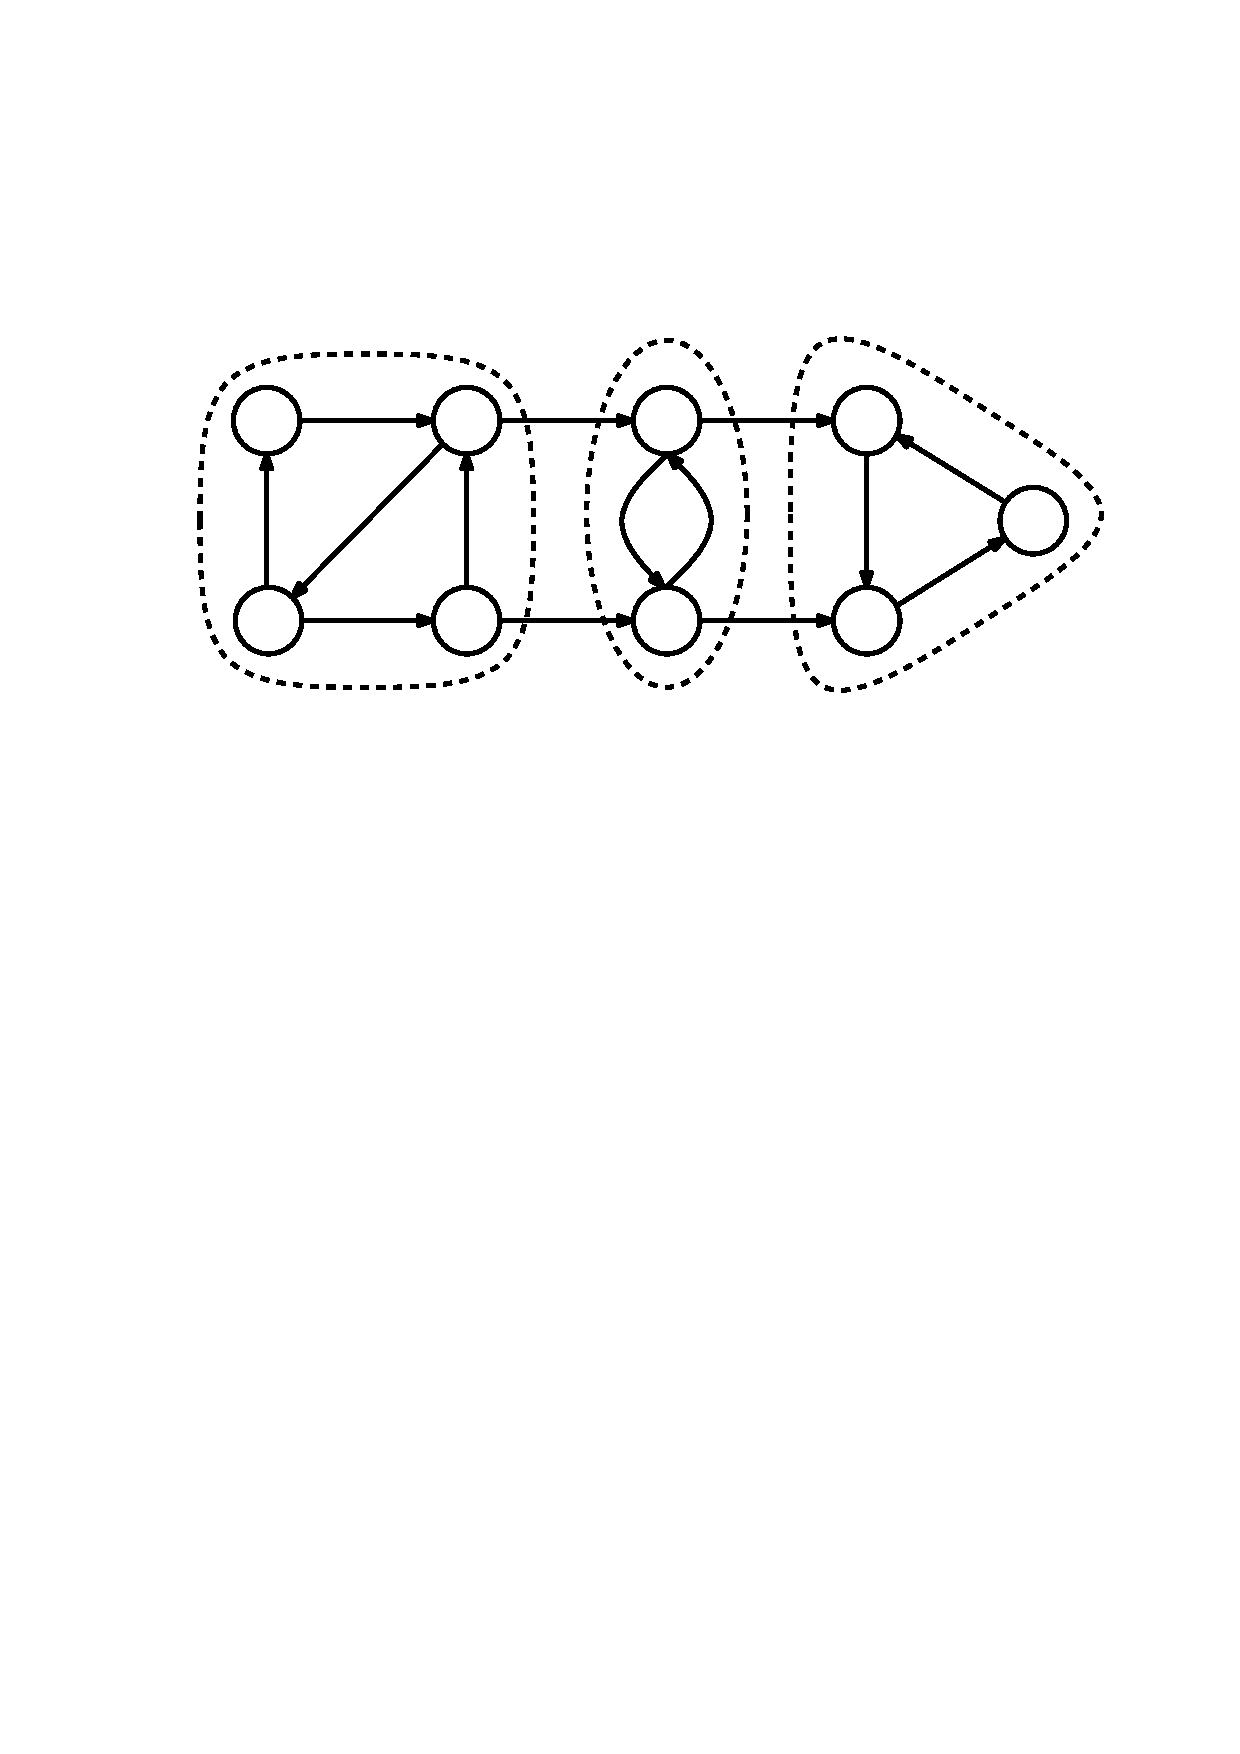
\includegraphics[scale=.5]{01_graph_theory/pics/strongly-connected_component.pdf}
	\caption{graph with 3 strongly connected components}
\end{figure}
\FloatBarrier

\begin{definition}
\index{shadow}
Let $G$ be a directed graph. The \dt{shadow} $H$ of $G$ is the undirected graph
that results when we ignore edge directions on $G$.
\end{definition}

\begin{definition}
\index{graph!connected!weakly}
$G$ is \dt{weakly connected} if its shadow $H$ is connected.
\end{definition}

\begin{definition}
\def\Gr{\ensuremath{G_\text{R}}}
\def\Vr{\ensuremath{V_\text{R}}}
\def\Er{\ensuremath{E_\text{R}}}
Let $G=(V,E)$ be a directed graph. Let
\[ K_1=\{v_1,\ldots\},K_2,\ldots,K_M \]
be the strongly connected components of $G$. Let $\Gr=(\Vr,\Er)$ with
\begin{align*}
\Vr &= \{K_1,\ldots,K_M\} \\
\Er &= \left\{(K_i,K_j) \mid \exists v\in V(K_i)\,\exists w\in V(K_j): (v,w)\in E\right\}.
\end{align*}
\index{reduction}%
Then we call $\Gr$ the \dt{reduction} of $G$.
\end{definition}

\textbf{Remark.} $G_\text{R}$ is always acyclic.

% strongly connected components
\begin{figure}[htb]
\resizebox{\textwidth}{!}{
\subfigure[directed Graph $G$]
{
	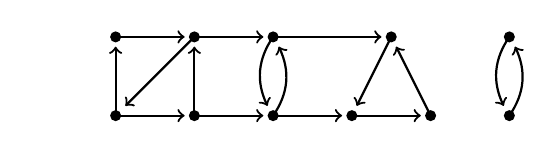
\begin{tikzpicture}
	\node at (0,0) {};
	\node (k1) at (1,0) {};
	\node (k2) at (2,0) {};
	\node (k3) at (2,1) {};
	\node (k4) at (1,1) {};

	\node (k5) at (3,0) {};
	\node (k6) at (3,1) {};

	\node (k7) at (4,0) {};
	\node (k8) at (5,0) {};
	\node (k9) at (4.5,1) {};

	\node (k10) at (6,0) {};
	\node (k11) at (6,1) {};

	\foreach \i in {1,...,11}
	{
		\fill (k\i) circle [radius=2pt];
	};

	\foreach \i / \j in {
	1/2, 2/3, 3/1, 4/3, 1/4,
	7/8, 8/9, 9/7,
	2/5, 3/6,
	5/7,
	6/9}
	{
		\path (k\i.center) edge[->, thick] (k\j);
	};
	\foreach \i / \j in {
	5/6, 6/5,
	10/11, 11/10}
	{
		\path (k\i.center) edge[->, thick, bend right] (k\j);
	};

	\end{tikzpicture}
}
\subfigure[shadow $H$ of Graph $G$]
{
	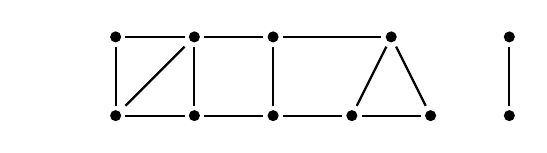
\begin{tikzpicture}
	\node at (0,0) {};
	\node (k1) at (1,0) {};
	\node (k2) at (2,0) {};
	\node (k3) at (2,1) {};
	\node (k4) at (1,1) {};

	\node (k5) at (3,0) {};
	\node (k6) at (3,1) {};

	\node (k7) at (4,0) {};
	\node (k8) at (5,0) {};
	\node (k9) at (4.5,1) {};

	\node (k10) at (6,0) {};
	\node (k11) at (6,1) {};

	\foreach \i in {1,...,11}
	{
		\fill (k\i) circle [radius=2pt];
	};

	\foreach \i / \j in {
	1/2, 2/3, 3/1, 4/3, 1/4,
	7/8, 8/9, 9/7,
	2/5, 3/6,
	5/7,
	6/9,
	5/6, 6/5,
	10/11, 11/10}
	{
		\path (k\i) edge[thick] (k\j);
	};
	\end{tikzpicture}
}}
\resizebox{\textwidth}{!}{
\subfigure[strongly connected components of $G$]
{
	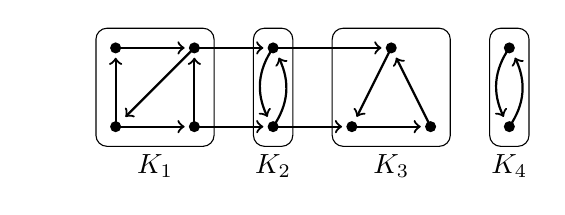
\begin{tikzpicture}
	\node at (0,0) {};
	\node (k1) at (1,0) {};
	\node (k2) at (2,0) {};
	\node (k3) at (2,1) {};
	\node (k4) at (1,1) {};

	\node (k5) at (3,0) {};
	\node (k6) at (3,1) {};

	\node (k7) at (4,0) {};
	\node (k8) at (5,0) {};
	\node (k9) at (4.5,1) {};

	\node (k10) at (6,0) {};
	\node (k11) at (6,1) {};

	\foreach \i in {1,...,11}
	{
		\fill (k\i) circle [radius=2pt];
	};

	\foreach \i / \j in {
	1/2, 2/3, 3/1, 4/3, 1/4,
	7/8, 8/9, 9/7,
	2/5, 3/6,
	5/7,
	6/9}
	{
		\path (k\i.center) edge[->, thick] (k\j);
	};
	\foreach \i / \j in {
	5/6, 6/5,
	10/11, 11/10}
	{
		\path (k\i.center) edge[->, thick, bend right] (k\j);
	};

	\draw[rounded corners] (0.75, -0.25) rectangle (2.25, 1.25);
	\draw[rounded corners] (2.75, -0.25) rectangle (3.25, 1.25);
	\draw[rounded corners] (3.75, -0.25) rectangle (5.25, 1.25);
	\draw[rounded corners] (5.75, -0.25) rectangle (6.25, 1.25);

	\node at (1.5, -0.5) {$K_1$};
	\node at (3.0, -0.5) {$K_2$};
	\node at (4.5, -0.5) {$K_3$};
	\node at (6.0, -0.5) {$K_4$};
	\end{tikzpicture}
}
\subfigure[reduction $G_R$ of Graph $G$]
{
	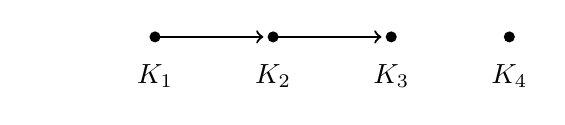
\begin{tikzpicture}
	\node at (0,0) {};
	\node (k1) at (1.5, 0) {};
	\node (k2) at (3.0, 0) {};
	\node (k3) at (4.5, 0) {};
	\node (k4) at (6.0, 0) {};

	\node at (1.5, -0.5) {$K_1$};
	\node at (3.0, -0.5) {$K_2$};
	\node at (4.5, -0.5) {$K_3$};
	\node at (6.0, -0.5) {$K_4$};

	\foreach \i in {1,...,4}
	{
		\fill (k\i) circle [radius=2pt];
	};
	\foreach \i / \j in {1/2, 2/3}
	{
		\path (k\i.center) edge[->, thick] (k\j);
	};
	\end{tikzpicture}
}}
\caption{Graphs}
\end{figure}





\begin{definition}
\index{node base}
Let $G$ be a directed graph. $B$ is a \dt{node base} of $G$ if:
\begin{compactitem}
\item $B\subseteq V$,
\item $\forall v\in V\,\exists w\in B: w \operatorname{S} v$, and
\item $B$ minimal w.\,r.\,t. $\subseteq$.
\end{compactitem}
\end{definition}

\index{node base}
\textbf{Remark.} The node base of $G$ can easily be constructed from a node
base of $G_\text{R}$. Let $\{K_1,\ldots,K_L\}\subseteq V_\text{R}$ be a node
base of $G_\text{R}$. Then
\[ \left\{\{b_1,\ldots,b_l\mid b_i\in V(K_i)\}\right\} \]
is the set of all node bases of $G$.

\index{node base}
$G_\text{R}$ has a single unique node base.

\index{node base}
\textbf{Remark.} The node base of $G_\text{R}$ (or acyclic graphs in general) is
\[ \{K\in V_\text{R}\mid d_{G_\text{R}}^{-}(K) = 0\}. \]



